% makale_orbit_bastirma_tr.tex — TÜRKÇE sürüm (REVTeX 4.2, PRAB stili)
% İngilizce kaynak: makale_orbit_bastirma.tex. Grafikler İngilizce kalır;
% caption'lar Türkçedir. Yeniden yapılandırma (2026-07): §III sonunda köprü;
% BBA §IV'te toplu (hizalama rotası buraya taşındı); §V iki engel (koşullanma,
% optik nefes) + CR-toplam + limit (BPM-ofset dejenerasyonu); NN tamamen
% çıkarıldı; lock-in ve nefes figürleri Ek'e taşındı.
\documentclass[aps,prab,reprint,superscriptaddress,nofootinbib]{revtex4-2}

\usepackage[T1]{fontenc}
\usepackage[utf8]{inputenc}
\usepackage{graphicx}
\usepackage{amsmath,amssymb}
\usepackage{bm}
\usepackage[colorlinks=true,linkcolor=blue,citecolor=blue,urlcolor=blue]{hyperref}

\begin{document}

\title{Bir proton EDM depolama halkasında kuadrupol-kaçıklık kaynaklı sahte EDM
sinyalinin yörünge tabanlı yöntemlerle bastırılması}

\author{I. Abedrabbo}
\affiliation{Istinye University, Istanbul, T\"urkiye}
\author{S. Hac{\i}\"omero\u{g}lu}
\affiliation{Istinye University, Istanbul, T\"urkiye}

\date{\today}


\begin{abstract}
Protonun elektrik dipol momentini (EDM) ölçmek için önerilen depolama
halkasında, birkaç mikronluk kuadrupol kaçıklıkları bir geometrik (Berry) faz
üzerinden gerçek bir EDM'i taklit eder; bu, hedef duyarlılık olan
$10^{-29}\,e\!\cdot\!$cm'in bin katına varan bir seviyededir. Referans tasarım
bunu, demet-tabanlı hizalama (BBA) ile bir \emph{dört-katlı} ölçümün birlikte
kullanımıyla denetler: kuadrupol polaritesinin her iki durumunda alınan
karşı-dönen demet farkı, makine iki polarite durumunda özdeş olduğunda etkiyi
iptal eder. Semplektik spin izleme kullanarak, tek başına standart yörünge
düzeltmesinin ne kadar ilerleyebileceğini soruyoruz. Sahte EDM, kaçıklığın iki
ayrı parçasına bağlıdır: kapalı yörüngeyi bozan bir \emph{antisimetrik} parça ve
yörüngenin neredeyse tepki vermediği bir \emph{simetrik} parça; engel ikincisidir
ve onu tek bir demetten geri çatacak yörünge inversiyonları ile genlik okumaları
hep başarısız olur (sıfır-arayan BBA ona ulaşır, ama yavaş ve girişimli olarak).
Karşı-dönen iki demetin yörünge tepkilerinin neredeyse zıt olduğunu, dolayısıyla
simetrik parçanın iki yörüngenin \emph{toplamında} taşındığını gösteriyoruz: bu
parça her iki demette de ve onların farkında (referans zincirin izlediği ayrım)
görünmezken toplamda tümüyle açığa çıkar. İki yörüngeyi birlikte düzeltmek bu
nedenle simetrik bileşene yalnızca yörüngeden ulaşır: kalibre bir referansa karşı,
ham $10~\mu$m'lik bir makinede gerçekçi $\%1$ $\beta$-vuruşunda,
karşı-dönen fark on beş tohum üzerinde medyan hedefin $0{,}043$ katına iner
(hepsi hedef-altı) ve $\beta$-vuruşuna ve modellenmemiş kuadrupol dönüklüğüne
duyarsızdır. Ne var ki aynı toplam statik BPM ofsetini de taşır; bu yüzden
simetrik kaçıklık ile ofset orada \emph{dejeneredir}: mutlak hizalama hâlâ tek bir
kalibrasyon kampanyası (BBA ya da dört-katlı) gerektirir ve bunu kesin biçimde
ortaya koyuyoruz. İki-demet düzeltmesinin ortadan kaldırdığı şey \emph{tekrarlanan}
kampanyadır: drift diferansiyeldir, statik ofset yörünge değişiminde iptal olur ve
sürekli bir iki-demet geri beslemesi, tek-demet geri beslemesinin göremediği
simetrik drifti ofset-serbest seviyede tutar. Rolü böylece, referans programın
gerektirdiği periyodik yeniden-hizalamanın yerine, başlangıç hizalamasını süresiz
koruyan sürekli bir simetrik-drift gözcüsüdür. Temel çizgi olarak dört-katlı
iptali doğruluyor ve ortaya çıkan işletme gereksinimlerini veriyoruz.
\end{abstract}

\maketitle

% ═══════════════════════════════════════════════════════════════════
\section{Giriş}
\label{sec:intro}

\subsection{Donmuş-spin yöntemi ve sahte-EDM problemi}
\label{sec:problem}

Protonun kalıcı bir elektrik dipol momenti (EDM), zamanı-tersine-çevirme
simetrisini ihlal eder ve Standart Model beklentisinin
($\lesssim 10^{-31}\,e\!\cdot\!$cm) üzerinde gözlenmesi, CP ihlalinin yeni
kaynaklarının doğrudan kanıtı olurdu. Önerilen depolama-halkası
deneyi~\cite{omarov}, \emph{donmuş-spin} yöntemiyle
$d = 10^{-29}\,e\!\cdot\!$cm duyarlılığını hedefler: protonlar ``sihirli''
momentumda ($p \approx 0{,}7$~GeV/$c$) depolanır; bu momentumda demet
dolaşırken spin momentumla hizalı kalır. Bir EDM, kendini radyal elektrik
büküm alanının sürüklediği yavaş bir spin dönmesiyle, spinin halka düzleminden
dışarı çıkması olarak açığa vurur. Ölçülen nicelik düzlem-dışı presesyon
hızıdır:
\begin{equation}
  f \equiv \frac{dS_y}{dt}, \qquad
  d = 10^{-29}\,e\!\cdot\!\text{cm} \;\leftrightarrow\;
  f \approx 1~\text{nrad/s}.
  \label{eq:target}
\end{equation}
Spini bu seviyede düzlem-dışına döndüren her rakip etki elenmeli ya da
sınırlanmalıdır; bu tür etkilere \emph{sahte EDM} sinyalleri denir.

Bu makalenin konusu, odaklayıcı kuadrupollerin enine kaçıklıklarının ürettiği
sahte EDM'dir; halkanın tümü-elektrik bir sürümü için Ref.~\cite{haciomeroglu2017}'de
incelenmiş ve Ref.~\cite{omarov}'un hata bütçesinin merkezinde yer alan bir
sistematiktir. Bir kuadrupolün manyetik ekseninde alanı sıfırdır; eksen-dışı geçen
bir demet, kaçıklıkla orantılı bir alan görür. Dikey bir $dy$ kaçıklığı demeti
radyal bir manyetik alana maruz bırakır; bu, spini radyal eksen etrafında
presesyona sokar ve dolayısıyla onu halka düzleminden dışarı eğebilir. Yatay bir
$dx$ kaçıklığı ise demeti dikey bir alana maruz bırakır; bu, spini dikey eksen
etrafında presesyona sokar; bu presesyon halka düzlemiyle sınırlıdır ve tıpkı
donmuş-spin koşulunun kendi düzlem-içi presesyonu gibi $S_y$'de birikmez. İki
presesyonun her biri tek başına neredeyse zararsızdır: halka boyunca ortalandığında
düzlem-dışı etkisi büyük ölçüde iptal olur. Ancak ikisi birden mevcut olduğunda, bu
presesyonlar yer değiştiremez (komütmez) --- önce radyal eksen etrafında sonra
dikey eksen etrafında presesyon, ters sıradaki işlemle aynı değildir --- ve bu
komütmezliğin artığı, EDM'in arandığı düzlem-dışı yön olan üçüncü eksen etrafında
net bir dönme olarak tur üzerine tur birikir. Bu bir geometrik (Berry) fazdır ve
başat bağımlılığı
\begin{equation}
  f_{\text{sahte}} \;\propto\; dx \cdot dy
  \;\;\Longrightarrow\;\;
  f_{\text{sahte}} \propto \sigma^2
  \label{eq:sigma2}
\end{equation}
şeklindedir; burada $\sigma$ kaçıklıkların rms büyüklüğüdür. Kuadratik ölçeklemeyi
Böl.~\ref{sec:estimator}'de doğrudan doğruluyoruz (ölçülen üs $p = 2{,}00 \pm 0{,}01$,
Ref.~\cite{omarov} Şek.~9(a) ile uyumlu). Gerçekçi bir $\sigma = 10~\mu$m
hizalamasında sahte EDM, Denk.~(\ref{eq:target}) hedefinin yaklaşık bin katıdır ve
gerçek sinyalle aynı gözlenebilirde, $dS_y/dt$, ortaya çıkar.

\subsection{Halka}
\label{sec:ring}

Burada incelenen kafes Ref.~\cite{omarov}'un simetrik-hibrit halkasıdır: elektrik
büküm, manyetik odaklama. Halka ($R_0 = 95{,}49$~m) 24 özdeş FODO hücresinden
oluşur. Her hücre bir yatay-odaklayan kuadrupol (QF) ile bir yatay-dağıtan
kuadrupol (QD) içerir --- ikisi de \emph{manyetik}, eşit büyüklükte ve zıt
işaretli gradyanlarla ($g \approx 0{,}2$~T/m) --- alansız sürüklenmeler ve
\emph{elektrik} büküm deflektörleriyle ayrılmış olarak:
\begin{align*}
  \text{QF} \to \text{sürükl.} \to \text{deflektör} \to \text{sürükl.} \to
  \text{QD} & \\
  {} \to \text{sürükl.} \to \text{deflektör} \to \text{sürükl.} \to
  (\text{QF}\ldots) &
\end{align*}
Deflektörler demeti yatay düzlemde büken silindirik elektrostatik
kapasitörlerdir; sihirli momentumda ($p = 700{,}7$~MeV/$c$, $\gamma = 1{,}248$,
$\beta = 0{,}598$) radyal alanları aynı zamanda düzlem-içi spin presesyonunu
dondurur. Sihirli koşul ve halka yarıçapının belirlediği radyal alan
$E_0 = \beta c\, (p/qR_0) \approx 4{,}4$~MV/m'dir (izleyicide kullanılan değer;
çevrenin bir kesrini kaplayan deflektörlerin içindeki yerel alan buna karşılık
daha büyüktür). Bu düzenlemenin sonrası için önemli iki özelliği var. Birincisi,
herhangi iki komşu kuadrupol arasında demet bir deflektörden geçer: deflektörler
demeti \emph{yatay} olarak büker ve zayıfça odaklarken, \emph{dikey} düzlemde çok
iyi bir yaklaşıklıkla alansız sürüklenmeler gibi davranırlar. İkincisi, izleyicide
deflektörler dahil edilerek tur-içi betatron salınımından ölçülen betatron tune
değerleri $Q_x = 2{,}64$ ve $Q_y = 2{,}30$'dur (tune, devir başına enine salınım
sayısıdır) --- bu kafesin modellendiği ama tam olarak yeniden üretmediği
Ref.~\cite{omarov}'un $2{,}70$ ve $2{,}245$ tasarım değerlerine yakın. Düzlemler
\emph{dejenere değildir}: deflektörlerin yatay odaklaması $Q_x$'i $Q_y$'nin
belirgin biçimde üstüne çıkarır; oysa deflektörleri her iki düzlemde sürüklenme
olarak ele alan analitik bir model her ikisine de $2{,}30$ verir ve ayrımı
kaçırır (Böl.~\ref{sec:bbareal}'in BBA yönlendirmesinde geri dönen bir olgu).
Böl.~\ref{sec:symanti}'nin yörünge kazanç yasasını belirleyen, dikey tune
$Q_y \approx 2{,}3$'tür; çünkü sahte EDM dikey düzlem üzerinden sürüklenir.

\subsection{Önerilen denetim programı ve bu makalenin sorusu}
\label{sec:remedy}

Ref.~\cite{omarov}'un tasarım çalışması bu sistematiği denetlemek için iki
bileşenli bir program zaten belirtir. Birincisi \emph{demet-tabanlı hizalamadır}
(BBA): hızlandırıcı topluluğu, kuadrupol gradyanını değiştirerek ve yörüngenin
tepki vermeyi bıraktığı demet konumunu bularak tek tek kuadrupol merkezlerini
konumlandırır; bu yordam ac uyarımla hızlandırılır~\cite{marti} ve çok sayıda
mıknatıs üzerinden paralelleştirilir~\cite{huang}. İkincisi bir \emph{dört-katlı
ölçümdür}: gerçek EDM demet-tersine-çevirme altında tektir, dolayısıyla iki
depolanan demetin karşı-dönen farkı onu ortak-mod sistematiklerden ayırır
[Ref.~\cite{omarov} Denk.~(C1)] ve bu farkı bütün odaklayıcı kuadrupollerin
polaritesi ters çevrilerek yinelemek [Denk.~(C2)] manyetik-kafes sahte EDM'ini tam
olarak iptal eder --- yeter ki makine her iki polarite durumunda aynı kaçıklığı
sunsun. Bu dört-katlı iptal güçlüdür ama bedelsiz değildir: iki polarite durumu
aynı anda depolanamaz, dolayısıyla deney ters polaritede ikinci kez
koşturulmalıdır ve Böl.~\ref{sec:fourfold}'de gösterdiğimiz gibi, iptal iki koşu
arasındaki herhangi bir hizalama değişimiyle bozulur.

Bu arka plana karşı doğal soru şudur: \emph{standart yörünge düzeltmesi} --- kapalı
yörüngeyi yönlendirme elemanlarıyla düzleştirmek, tepki matrisinin tekil-değer
ayrışımıyla yönlendirilir, Chung, Decker ve Evans~\cite{chung1993} çalışmasından
beri rutin, veri alımı sırasında sürekli ve girişimsiz --- ne katkı sağlayabilir?
Kapalı yörünge, 48 kuadrupolün her birinde konumlanan demet-konum monitörleriyle
(BPM) okunur; ilgili araçlar arasında dejenerasyon altında yörünge-tepki
modelleme~\cite{wegscheider}, simetri düzeltmesi~\cite{mirza} ve çevrimiçi
tepki-matrisi iyileştirmesi~\cite{ziemann} bulunur. Bu tekniklerin hiçbiri
başlıbaşına yeni değildir. İncelediğimiz şey, her birinin bu halkadaki sahte
EDM'i sürükleyen belirli kaçıklık bileşeninde nasıl performans gösterdiğidir ve
sonuç doğal beklentinin tersine dönmesidir: tek-demet hiçbir yörünge ölçümü o
bileşene ulaşamazken, iki karşı-dönen demeti birlikte düzeltmek ulaşır; çünkü
simetrik kaçıklık iki yörüngenin toplamında yaşar. Aynı toplam statik BPM ofsetini
de onunla dejenere biçimde taşır, dolayısıyla iki-demet düzeltmesi tek-seferlik
mutlak hizalamanın yerini almaz --- ama \emph{tekrarlanan} hizalamanın yerini
alır, simetrik hizalamayı drifte karşı korur; bunu tek-demet geri beslemesi
yapamaz.

\subsection{Bulgular ve genel akış}
\label{sec:outline}

Makaleyi üç sonuç düzenler.

Birincisi, \emph{sahte EDM'in tek bir hizalama toleransının yakalayamayacağı bir
yapısı vardır} (Böl.~\ref{sec:mechanism}). O, yatay ve dikey kaçıklık
desenlerinin bilineer bir fonksiyonelidir ve her desen bir \emph{antisimetrik}
bileşene (komşu QF ve QD zıt yönde kaymış), ki büyük bir yörünge bozulması üretir,
ve bir \emph{simetrik} bileşene (QF ve QD birlikte kaymış), ki yörünge imzası mod
mod iki büyüklük mertebesine varan ölçüde bastırılmıştır, ayrılır. Sabit rms
$\sigma$'da sahte EDM, kaçıklığın hangi bileşeni taşıdığına göre bir büyüklük
mertebesinden fazla değişir.

İkincisi, \emph{referans çözüm hedefe ulaşır ama bir işletme bedeliyle}
(Böl.~\ref{sec:bba}). Demet-tabanlı hizalama simetrik bileşene ulaşır ve yeterince
yinelendiğinde hedefe tek başına da varır (izlememizde sekiz geçiş), ama yavaşça;
Ref.~\cite{omarov}'un dört-katlı polarite ölçümü bunun yerine sahte EDM'i tek
adımda iptal eder. İkisini de yeniden üretiyoruz. Bedel işletmeseldir: dört-katlı,
makinenin aynı simetrik hizalamayı sunduğu ardışık iki polarite durumu gerektirir
ve aralarındaki, yörüngeye görünmez, mikron ölçekli bir simetrik drift sahte EDM'i
yeniden açar.

Üçüncüsü, \emph{karşı-dönen yörünge düzeltmesi simetrik bileşene yörüngeden ulaşır
ve doğal rolü sürekli bir simetrik-drift gözcülüğüdür} (Böl.~\ref{sec:orbitreach}).
Tek-demet bir yörünge ölçümü simetrik bileşene ulaşamaz: o, tek demete neredeyse
görünmezdir ve onu geri çatacak inversiyon kötü koşulludur. Ama iki karşı-dönen
demetin yörünge tepkileri neredeyse zıttır, dolayısıyla simetrik bileşen --- her
iki demette de ve referans zincirin izlediği farklarında (ayrım) görünmezken ---
onların \emph{toplamında} tümüyle açığa çıkar. İki yörüngeyi kalibre bir referansa
karşı birlikte düzeltmek bu nedenle ona ulaşır, gerçekçi optik hatası ve dönüklükte
hedef-altında. Ne var ki aynı toplam statik BPM ofsetini simetrik kaçıklıkla orada
dejenere biçimde taşır, dolayısıyla mutlak hizalama hâlâ tek bir kalibrasyon
kampanyası gerektirir. İki-demet düzeltmesinin kaldırdığı şey \emph{tekrarlanan}
olandır: drift diferansiyeldir, ofset yörünge değişiminde iptal olur ve sürekli bir
iki-demet geri beslemesi simetrik hizalamayı --- tek-demet geri beslemesinin
tutamadığı bileşeni --- drifte karşı süresiz korur.

Kısaca yol haritası: problem ve mekanizma (Böl.~\ref{sec:mechanism}) simetrik
bileşene ulaşmayı zorunlu kılar; bunu önce mekanik olarak yapan referans çözüm
(BBA + dört-katlı, Böl.~\ref{sec:bba}), sonra yörüngeden yapan karşı-dönen toplam
(Böl.~\ref{sec:orbitreach}) gelir; ardından işletme (Böl.~\ref{sec:operation}) ve
sonuçlar (Böl.~\ref{sec:conclusions}). Tüm nicel ifadelerin dayandığı simülasyon
altyapısı ve spin-sinyali kestiricisi önce Böl.~\ref{sec:method}'de anlatılır.

% ═══════════════════════════════════════════════════════════════════

\section{Simülasyon yöntemi}
\label{sec:method}

\subsection{İzleme araçları}
\label{sec:tools}

Bütün sonuçlar, Böl.~\ref{sec:ring} kafesinin alanları boyunca hareket
denklemlerini eleman-eleman dördüncü-derece Gauss--Legendre semplektik
integratörüyle integre eden bir parçacık-ve-spin izleme koduyla elde edilir; spin
aynı adımlarda Thomas-BMT denklemiyle taşınır. Semplektik integrasyon, enerji ve
genlik hatalarının yavaş birikimini önler; bu, milyonlarca tur boyunca nrad/s
seviyesinde presesyon hızlarını çözebilmenin bir önkoşuludur. Gerçek EDM modele
bir anahtarla girer; kuplaj $\eta = 1{,}88\times10^{-15}$'e ayarlandığında kod,
demet-tersine-çevirme altında tek olan $dS_y/dt = 9{,}81\times10^{-10}$~rad/s'yi
üretir; bu, Ref.~\cite{omarov} Denk.~(C1) ile uyumludur. Aşağıdaki tüm sahte-EDM
sonuçları EDM anahtarı kapalıyken elde edilir, öyle ki ölçülen herhangi bir
düzlem-dışı presesyon inşa gereği bir sistematik etkidir. Kuadrupol kaçıklıkları,
gradyan hataları ($\beta$-vuruşu) ve dönüklük açıları izleyiciye doğrudan eleman
parametreleri olarak girer.

Geniş parametre taramaları (gürültü Monte Carlo, $\beta$-vuruşu süpürmeleri) ikinci,
bağımsız bir katman kullanır: kafes fonksiyonları, tune değerleri ve yörünge tepki
matrisi,
\begin{equation}
  R_{ij} = \frac{\sqrt{\beta_i\beta_j}}{2\sin\pi Q}\,(KL)_j
  \cos\!\big(|\phi_i-\phi_j| - \pi Q\big),
  \label{eq:R}
\end{equation}
kuadrupol ve sürüklenme transfer matrislerinden kapalı biçimde hesaplanır. Bu
analitik katman saniyeler içinde çalışır, dikey düzlemde izleyiciyle yüzde
seviyesinde uyuşur ve konfigürasyon dosyası dışında onunla hiçbir şey paylaşmaz,
böylece ikisi arasındaki uyum ortak bir uygulama hatasından doğamaz. İki
kısıtlaması sonrasında rol oynar ve burada kaydedilir: elektrik deflektörlerini
alansız sürüklenmeler olarak ele alır (dikeyde doğru, yatayda değil,
Böl.~\ref{sec:bba}); ve idealize bir tepki matrisi gerçek demet dinamiğini yanlış
temsil edebilir, dolayısıyla bir tepki matrisi nicel olarak girdiği her yerde ---
hem Böl.~\ref{sec:obstructions}'ün ters problemlerinde hem
Böl.~\ref{sec:bba}'nın BBA yönlendirmesinde --- izlemeden yeniden inşa edilir ve
bunun talep ettiği doğruluk bizzat sonuçlarımızdan biridir (Böl.~\ref{sec:bbareal}).

\subsection{Sahte EDM'in ölçülmesi}
\label{sec:estimator}

İlgilenilen nicelik $S_y(t)$'nin sekuler eğimidir. Onu güvenilir biçimde çekmek
dikkat gerektirir, çünkü izlenen parçacığın betatron salınımı, spin hareketine
aranan eğimi büyüklük mertebeleriyle aşan salınımlı bileşenler besler. İki önlem
birleştirilir.

Birincisi, izlenen parçacık, hiçbir betatron salınımının bulunmadığı kapalı yörünge
üzerine yerleştirilir. Kaçıklıkla-bozulmuş kapalı yörünge birkaç adımda Newton
yinelemesiyle bulunur.

İkincisi, spin geçmişi
$S_y(t) = a + bt + \sum_k \left[c_k\cos\omega_k t + d_k\sin\omega_k t\right]$
modeliyle uydurulur ve yalnızca sekuler eğim $b$ tutulur; kalan salınımlı içerik,
düz bir polinom uydurmasında olacağı gibi eğimi saptırmak yerine harmonik terimlerce
soğurulur.

Kestirici üç bağımsız yolla doğrulandı: (i) $\sigma = 2{,}5$--$10~\mu$m taraması
$|f| \propto \sigma^{p}$ verir, $p = 2{,}00 \pm 0{,}01$; bu, doğrusal kaçak
olmaksızın bir geometrik fazın saf kuadratik ölçeklemesidir; özellikle, yörünge
düzeltmesinden sonra $\sigma = 5~\mu$m'de $f = 0{,}62 \times 10^{-9}$~rad/s
ölçüyoruz (3 rasgele tohum medyanı), $\sigma = 10~\mu$m'deki
$2{,}72 \times 10^{-9}$~rad/s'ye karşı; bu, gözlenen $4{,}36$ oranını verir ve
$\sigma^2$ öngörüsü $4{,}0$ ile uyumludur; (ii) kaçıklık deseninin işaret
çevrimlerinde ölçülen $f$, $f(+dx,-dy) = -f(+dx,+dy)$ ve
$f(-dx,-dy) = +f(+dx,+dy)$'yi $10^{-3}$ seviyesinde sağlar, bu da
Denk.~(\ref{eq:sigma2})'nin bilineer karakterini doğrular; (iii) kapalı yörünge
çevresinde simetrik fırlatılan dört parçacığın ortalaması, tek yörünge-üstü sonucu
$\%1$ içinde yeniden üretir.\footnote{Simetrik dört-parçacık ortalaması kapalı
yörünge çevresinde kurulmalıdır; ideal eksen çevresinde kurulursa yörünge ofsetinin
bizzat indüklediği ortak betatron bileşenini korur ve büyüklük mertebeleriyle
başarısız olur.}

% ═══════════════════════════════════════════════════════════════════

\section{Sahte EDM: mekanizma ve kanallar}
\label{sec:mechanism}

Denk.~(\ref{eq:sigma2})'nin sahte EDM'i, desenin kaçıklığın hangi parçasını
taşıdığıyla belirlenir, yalnızca rms'iyle değil. Bu bölüm bunu kesinleştirir: her
kaçıklık düzlemini keskin biçimde farklı yörünge görünürlüğüne sahip bir simetrik
ve bir antisimetrik bileşene ayırır ve sahte EDM'in, dört kanalı antisimetrik
çarpanlarca domine edilen, iki düzlemde bilineer bir form olduğunu gösterir. Bu
yapı --- herhangi bir düzeltme şemasına atıf yapmadan burada kurulmuştur --- sonraki
her yöntemin baş etmesi gereken şeyi belirler: antisimetrik parça görülmesi ve
kaldırılması kolaydır, simetrik parça ikisi de değildir.

\subsection{Simetrik ve antisimetrik kaçıklıklar}
\label{sec:symanti}

Bir düzlemin 48 ofseti bir $v$ vektörü oluştursun; $k$ hücresinde QF $2k$
indisinde, QD $2k{+}1$ indisinde olsun. Bir hücre içinde iki ofset, kuadrupollerin
\emph{birlikte} hareket ettiği parça ile \emph{zıt} hareket ettiği parçaya
ayrılabilir --- çift üzerinde basit bir $2\times2$ işlemi:
\begin{align}
  \begin{pmatrix} v^{\rm s}[2k] \\ v^{\rm s}[2k{+}1] \end{pmatrix}
    &= \frac12\begin{pmatrix} 1 & 1 \\ 1 & 1 \end{pmatrix}
       \begin{pmatrix} v[2k] \\ v[2k{+}1] \end{pmatrix},
  \nonumber\\[4pt]
  \begin{pmatrix} v^{\rm a}[2k] \\ v^{\rm a}[2k{+}1] \end{pmatrix}
    &= \frac12\begin{pmatrix} 1 & -1 \\ -1 & 1 \end{pmatrix}
       \begin{pmatrix} v[2k] \\ v[2k{+}1] \end{pmatrix} .
  \label{eq:projectors}
\end{align}
İlk matris her iki ofseti ortalamalarıyla
$\tfrac12\big(v[2k]+v[2k{+}1]\big)$ değiştirerek simetrik parça $v^{\rm s}$'yi
verir; ikincisi onları farklarının $\pm$ yarısıyla
$\tfrac12\big(v[2k]-v[2k{+}1]\big)$ değiştirerek antisimetrik parça $v^{\rm a}$'yı
verir. Tam projektörler $P_{\rm sym}$ ve $P_{\rm anti}$, bu aynı $2\times2$ bloğunu
sırayla 24 hücrenin her birine uygular (öyle ki $v^{\rm s} = P_{\rm sym}v$ ve
$v^{\rm a} = P_{\rm anti}v$); tamamlayıcıdırlar, $P_{\rm sym}+P_{\rm anti}=I$. Aynı
matris çifti yatay ve dikey ofset vektörlerine bağımsız olarak uygulanır.

Bunu 24 hücre için yapmak, bir düzlemin 48 ofsetini 24 simetrik sayı
$m_k = \tfrac12\big(v[2k]+v[2k{+}1]\big)$ ve 24 antisimetrik sayı
$d_k = \tfrac12\big(v[2k]-v[2k{+}1]\big)$ olarak yeniden ifade eder. Orijinaller
$v[2k] = m_k + d_k$ ve $v[2k{+}1] = m_k - d_k$ ile geri kazanıldığından, bu hiçbir
şey kaybetmeyen tersinir bir yeniden etiketlemedir ($24 + 24 = 48$): simetrik desen
$v^{\rm s} = P_{\rm sym}v$ $m_k$'ları toplar (tüm $d_k = 0$), antisimetrik desen
$v^{\rm a} = P_{\rm anti}v$ $d_k$'ları toplar (tüm $m_k = 0$) ve her kaçıklık
vektörü tam olarak birer tanesinin toplamıdır, $v = v^{\rm s} + v^{\rm a}$. İki
desen ailesi ortogonaldir ve her biri 48-boyutlu kaçıklık uzayının yarısını gerer,
böylece \emph{herhangi} bir desenin çözüldüğü tam bir baz çifti oluştururlar; iki
düzleme ayrı ayrı uygulandığında bu, $v_x = v_x^{\rm s} + v_x^{\rm a}$ ve
$v_y = v_y^{\rm s} + v_y^{\rm a}$'yı verir; bu, Böl.~\ref{sec:bilinear}'in kanal
ayrışımında kullanılan gösterimdir.

İki bileşen arasındaki fiziksel ayrım, QF ile QD'nin zıt-işaretli gradyanlarından
gelir. Kaçık bir kuadrupol demeti (gradyan)$\times$(ofset) ile orantılı bir açıyla
saptırır. İki komşu \emph{zıt} yönde kaydığında (antisimetrik bileşen), zıt
gradyanlar ve zıt ofsetler \emph{aynı} işaretli tekmelere birleşir: tekmeler halka
boyunca, başat azimutal harmonikleri betatron tune'a yakın olan yavaş değişen bir
saptırma desenine tutarlı biçimde eklenir ve kapalı-yörünge tepkisi büyüktür. İki
komşu \emph{birlikte} kaydığında (simetrik bileşen), tekmeler zıttır ve her hücre
içinde iptal olur; hayatta kalan şey azimutal harmonik $k \approx 24$'te bir
hücre-hücre alternasyondur (hücre başına bir işaret değişimi, 24 hücre). Harmonik
$k$'lı bir saptırma desenine kapalı-yörünge tepkisi kazanç yasasını izler,
\begin{equation}
  G_k = \frac{C}{|Q^2 - k^2|}, \qquad C \approx 24{,}8,\; Q^2 \approx 5 ,
  \label{eq:Gk}
\end{equation}
ki bu, tune'a yakın $k$ için rezonanstır ve çok üstünde güçlü biçimde
bastırılmıştır; $Q \approx 2{,}3 \ll 24$ ile simetrik bir bileşenin alternans
saptırma deseni neredeyse görünmezdir [Şek.~\ref{fig:modes}]. Nicel olarak,
$10$-$\mu$m-rms'lik rasgele bir desen, antisimetrikse $\sim\!100~\mu$m ama
simetrikse $\sim\!19~\mu$m rms yörünge izi bırakır (izlemeden türetilen tepki) ve
iki iz yalnızca büyüklükte değil türde de farklıdır: simetrik iz neredeyse tümüyle
\emph{kaçaktır}, desenin güçlü-kuplajlı modlara birkaç-yüzdelik bir karışımı.
Yörünge düzeltmesi bu nedenle antisimetrik bir desenin ürettiğinin çoğunu iptal
eder ama simetrik olanın yalnızca o birkaç-yüzdelik kaçağına ulaşır --- simetrik
kaçıklığın kendisi neredeyse dokunulmadan kalır ve onunla birlikte artık sahte EDM.

\begin{figure*}[tb]
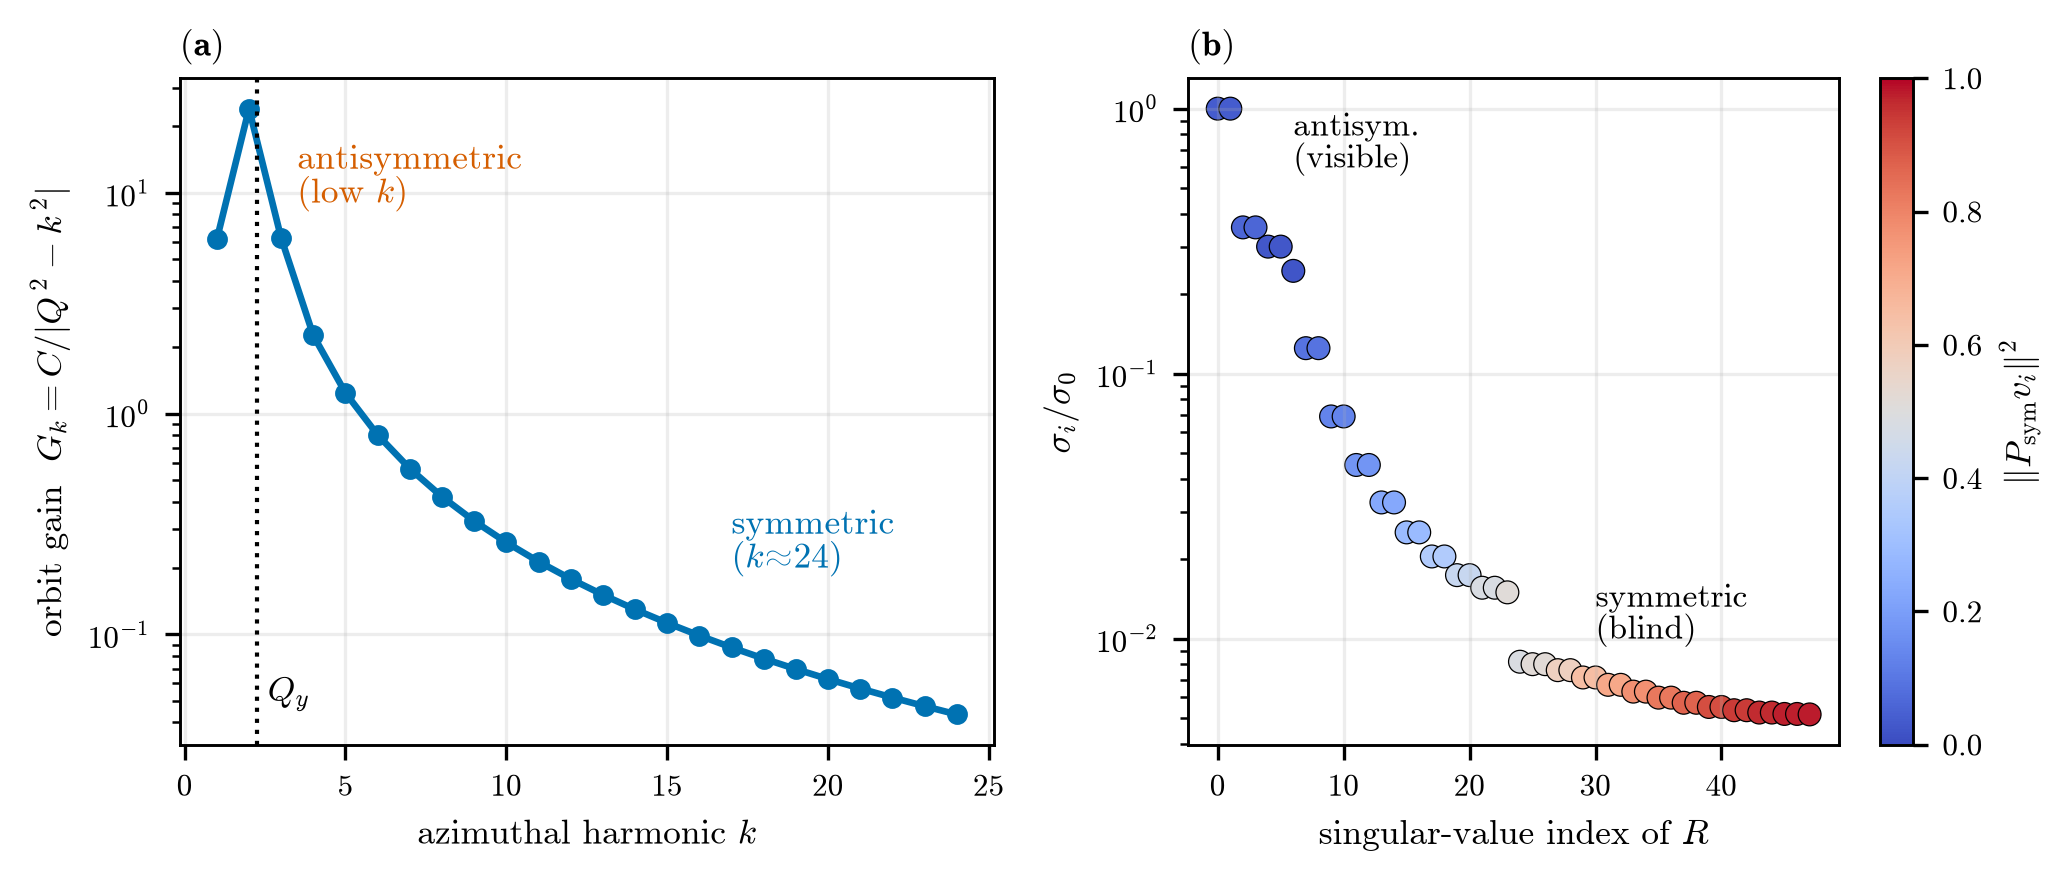
\includegraphics[width=0.95\textwidth]{fig_orbit_modes.png}
\caption{Kaçıklık desenlerinin yörünge görünürlüğü (analitik kafes,
$Q_y = 2{,}30$). Sol: Denk.~(\ref{eq:Gk})'nin yörünge kazanç yasası; antisimetrik
desenler betatron rezonansına yakın düşük harmonikleri sürükler, simetrik desenler
çok üstündeki $k\approx24$'ü sürükler. Sağ: bağımsız kaçıklık desenleri yörünge
tepkilerinin gücüne göre sıralanmış; güçlü kuplajlananlar antisimetriktir (QF, QD
zıt), zayıf kuplajlananlar simetriktir (QF, QD birlikte); görünürlük oranı
$\mathrm{cond}(R)=193$'tür.}
\label{fig:modes}
\end{figure*}

\subsection{Bilineer form olarak sahte EDM: dört kanal}
\label{sec:bilinear}

Bu ayrışım ile sahte EDM arasındaki bağ, ek bir formalizm olmaksızın doğrudan
Böl.~\ref{sec:problem}'in fiziğinden gelir. Yatay kaçık bir kuadrupol, spini dikey
eksen etrafında ofseti $v_{x,i}$ ile orantılı küçük bir açıyla presesyona sokar;
dikey kaçık bir kuadrupol onu radyal eksen etrafında $v_{y,j}$ ile orantılı bir
açıyla presesyona sokar. Farklı eksenler etrafındaki iki presesyon komütmez ve her
sıralı çiftin bıraktığı düzlem-dışı artık iki küçük açının \emph{çarpımıyla}
orantılıdır. Bunu halka boyunca tüm kuadrupol çiftleri üzerinden toplayınca,
\begin{equation}
  f \;=\; \sum_{i}\sum_{j} W_{ij}\; v_{x,i}\, v_{y,j}
  \;\equiv\; B(v_x, v_y),
  \label{eq:bilinear}
\end{equation}
elde edilir; burada ikili ağırlıklar $W_{ij}$ yalnızca kafese bağlıdır --- iki
mıknatısın nerede oturduğuna ve birinin başlattığı yörünge saptırmasının diğerine
halka boyunca nasıl taşındığına [yörünge tepkisi, Denk.~(\ref{eq:R})] --- ve
kaçıklıkların kendilerine değil. Denk.~(\ref{eq:bilinear}) sahte EDM'in
\emph{bilineer} olduğunu söyler: her terim tam olarak bir yatay ve bir dikey ofset
içerir, asla aynı düzlemden iki tane değil. Bu, Böl.~\ref{sec:estimator}'de
doğrudan doğrulanan işaret yapısıdır.

Her düzlemi bağımsız olarak simetrik ve antisimetrik parçalarına ayırıp,
$v_x = v_x^{\rm s} + v_x^{\rm a}$ ve $v_y = v_y^{\rm s} + v_y^{\rm a}$
[Denk.~(\ref{eq:projectors})], ve çift toplamı açınca, terimler dört gruba düşer:
\begin{equation}
  f = \underbrace{B(v_x^{\rm s},v_y^{\rm s})}_{f_{ss}}
    + \underbrace{B(v_x^{\rm s},v_y^{\rm a})}_{f_{sa}}
    + \underbrace{B(v_x^{\rm a},v_y^{\rm s})}_{f_{as}}
    + \underbrace{B(v_x^{\rm a},v_y^{\rm a})}_{f_{aa}} .
  \label{eq:channels}
\end{equation}
İki düzlem projektörlerce değil, ağırlıklar $W_{ij}$ ile karışır. Bir kaçıklık
bileşeni spine esasen sürüklediği yörünge üzerinden etki ettiğinden ve bu yörünge
antisimetrik bir bileşen için büyük, simetrik bir bileşen için $G_k$-bastırılmış
olduğundan [Denk.~(\ref{eq:Gk})], saf-simetrik kanal $f_{ss}$ açık ara en küçüktür
ve antisimetrik çarpan içeren her kanal daha büyüktür.

$f_{sa}$ ve $f_{as}$'nin çifte-sayım değil, iki ayrı fiziksel nicelik olduğunu
vurguluyoruz. $f_{sa}$'da \emph{yatay} desen simetriktir ve \emph{dikey} olan
antisimetriktir; $f_{as}$'de roller değişir. Hiçbir şey bunları eşit olmaya
zorlamaz: iki düzlem halkaya farklı girer (yalnızca yatay düzlem bükümü taşır) ve
ağırlıklar $W_{ij}$ düzlemlerin değişimi altında simetrik değildir, çünkü komütmeyen
iki presesyonun sırası önemlidir. İzleyici farkı doğrudan doğrular: temsili desen
için $f_{as} = -272\times$ hedef iken $f_{sa} = +28\times$ --- bir büyüklük
mertebesi aralıkta ve zıt işaretli.

Her kanal bir uydurma değil, ayrı bir izleme ölçümüdür ve bu ölçüm, bu makaledeki
bütün simetrik/antisimetrik atıflarının temelini oluşturur. Kaçıklık deseni
$(v_x, v_y)$ Denk.~(\ref{eq:projectors}) ile bir kez izdüşürülür ve izleyici sonra
dört kez koşturulur. Her koşuda makinenin kuadrupol ofsetleri düzlem başına bir
izdüşürülmüş parçaya \emph{ayarlanır} --- örneğin $f_{as}$ için yatay ofsetler
$v_x^{\rm a}$ deseni ve dikey ofsetler $v_y^{\rm s}$'dir, başka kusur yok --- ve
Böl.~\ref{sec:estimator}'in kestiricisi o kanalın $f$'ini doğrudan verir. Ağırlıklar
$W_{ij}$'nin bilinmesi ya da hesaplanması hiç gerekmez: onlar izleyicinin bizzat
cisimleştirdiği kafes özellikleridir ve Denk.~(\ref{eq:bilinear}) yalnızca her
terimin tam olarak bir yatay ve bir dikey ofset içerdiği yapısal sonucu üzerinden
girer, öyle ki dört koşu terimlerin dört grubunu ayırır. Bilineerlik böylece
varsayılmak yerine sınanır: Şekil~\ref{fig:channels} sonucu $\sigma = 10~\mu$m'de
gösterir: dört işaretli kanal tam-desen sahte EDM'ine $\%0{,}1$ içinde toplanır
(üç tohum üzerinde $f/\!\sum = 0{,}999$--$1{,}001$), Denk.~(\ref{eq:channels})'i
doğrulayarak; saf-simetrik kanal her tohumda en küçüktür; ve her kanal ayrı ayrı
$\sigma^{2}$ olarak ölçeklenir. Ölçülen kanal oranları bilineer yapıyla tutarlıdır:
düzlem başına $\sim\!5$'lik bir yörünge-izi çarpanı girer, dolayısıyla onlarca
mertebesinde bir $f_{aa}/f_{ss}$ beklenir ve gözlenir. Ölçülen kanallar boyunca
nicel referans olarak kullanılır.

İki sonuç makalenin geri kalanını çerçeveler. Birincisi, sahte EDM rms kaçıklığın
bir fonksiyonu değildir: $\sigma^{2}$-homojendir, ama sabit $\sigma$'da değeri desene
bağlıdır --- Şek.~\ref{fig:channels}'de aynı $10~\mu$m rms'te kanal büyüklükleri üç
tohum ortalamalarında ${\sim}20\times$'ten ${\sim}400\times$ hedefe, tek tohumlar
arasında ${\sim}1\times$'ten ${\sim}900\times$'e uzanır. Bu yüzden tek bir hizalama
toleransı sistematiği özetleyemez ve bir düzeltme yordamı kaçıklığın yalnızca
büyüklüğünü değil \emph{istatistiğini} değiştirir: rasgele bir deseni, yordamın
göremediği bileşende yoğunlaşmış yapılı bir desene çevirir. İkincisi, bastırma için
işbölümü Denk.~(\ref{eq:channels}) ile sabittir: yörünge düzeltmesi antisimetrik
çarpanları ve onlarla üç büyük kanalı kaldırır; kalan taban $f_{ss}$'tir ve daha
ileri her ilerleme simetrik bileşenin kendisine ulaşan bir ölçüm gerektirir.
\emph{Dolayısıyla başarılı her düzeltme şeması simetrik bileşen hakkındaki bilgiyi
geri kazanmalıdır.}

\begin{figure*}[tb]
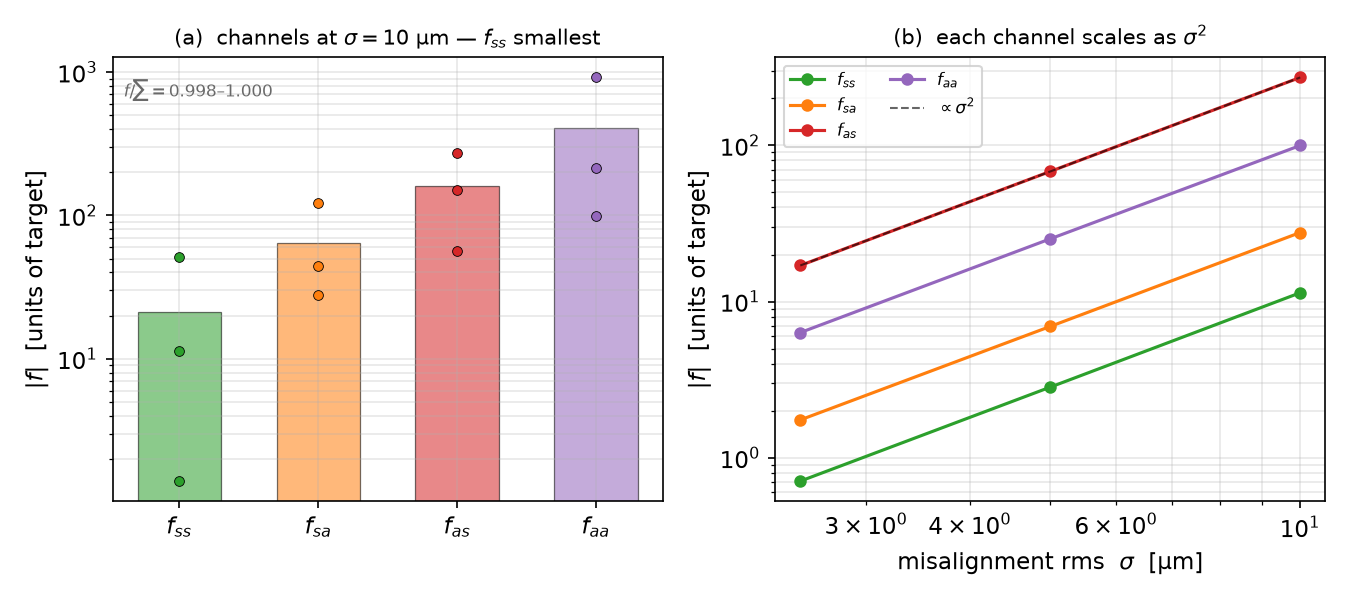
\includegraphics[width=0.9\textwidth]{fig_orbit_channels.png}
\caption{Denk.~(\ref{eq:channels})'in dört sahte-EDM kanalı, kaçıklıklar
izdüşürülüp her parça ayrı izlenerek ölçülmüş. (a) $\sigma=10~\mu$m'de
saf-simetrik kanal $f_{ss}$ en küçüktür ve antisimetrik çarpan içeren her kanal
daha büyüktür (işaretler: tek tek tohumlar; yatay çizgi: ortalamaları; yayılım
$f$'in işaretli, bilineer karakterini yansıtır). (b) Her kanal $\sigma^2$ olarak
ölçeklenir. Dört işaretli kanal tam sinyale $\%0{,}1$ içinde toplanır.}
\label{fig:channels}
\end{figure*}

% ═══════════════════════════════════════════════════════════════════

\section{Simetrik bileşeni mekanik olarak geri kazanmak: referans çözüm ve bedeli}
\label{sec:bba}

Ref.~\cite{omarov}'un tasarım çalışması simetrik kaçıklığı iki bileşenle denetler:
yörünge inversiyonunun ulaşamadığı simetrik bileşene ulaşan demet-tabanlı hizalama
(BBA) ve artık sahte EDM'i iptal eden dört-katlı polarite ölçümü. İkisini de
izlemede yeniden üretiyor, sonra her birinin bedelini nicelendiriyoruz. Ortaya
çıkan tablo --- BBA hedefe ama ancak çok geçişten sonra ulaşır, dört-katlı bir
kerede ulaşır ama yalnızca makine ardışık bir polarite tersine-çevirmesi boyunca
özdeş tutulursa --- Böl.~\ref{sec:orbitreach}'in yalnız-yörünge alternatifini
motive eden şeydir.

\subsection{Yordam}
\label{sec:bbaproc}

Standart kuadrupol demet-tabanlı hizalaması bir matris tersine almaz ve bir
kalibrasyona karşı genlik okumaz; her manyetik merkezi, bir gradyan değişimine
tepkinin \emph{sıfırlandığı} demet konumu olarak konumlandırır. Hizalanabilir 47
kuadrupolün her biri için sırayla:\footnote{Hücre 0'ın gradyan-modülasyonlu
kuadrupolü modelimizde ayrı bir eleman tipidir ve dışlanır; ofseti sıfıra ayarlanır
ve öyle raporlanır.} (i) tek tepki-matrisi elemanı $R_{ij}$ ile ölçeklenen en yakın
yönlendirme düzelticisiyle demet, $i$ kuadrupolünün beklenen merkezini kuşatan iki
konuma yerleştirilir; (ii) her konumda $i$ kuadrupolünün gradyanı küçük bir miktar
değiştirilir ve iki kapalı yörüngenin farkı 48 BPM'nin hepsinde kaydedilir --- bu
fark, demet--merkez ofsetiyle orantılı feed-down izidir; (iii) demet merkezi
geçtikçe iz işaret değiştirdiğinden, merkez BPM'ler üzerinde ağırlıklı en-küçük-kareler
sıfırı olarak elde edilir; BPM başına sıfır geçişlerinin yayılımı mıknatıs-başına bir
kalite ölçüsü olarak tutulur. Bütün yörüngeler demet 4B kapalı yörünge üzerine
yerleştirilerek okunur (Böl.~\ref{sec:estimator}). Simülasyonda yönlendirme
düzelticisi, sınanan kuadrupole komşu bir kuadrupolün denetimli enine yer
değiştirmesidir; deneyde aynı dipol tekme, herhangi bir mıknatıs oynatılmadan,
kuadrupol bobinleri arasındaki bir akım asimetrisiyle üretilebilir; bu, manyetik
merkezi elektriksel olarak kaydırır. İkisi eşdeğerdir --- ofsetli bir kuadrupol ile
üzerine bindirilmiş dipol alanlı eksen-üstü bir kuadrupol, hem yörünge hem spin
üzerinde özdeş davranır.

Bu yordamda tepki matrisinin rolü \emph{ileri} yönle sınırlıdır: tek, iyi-koşullu
bir eleman yönlendirme tümseğini boyutlandırır. Hiçbir yerde global bir ters
görünmez, dolayısıyla Böl.~\ref{sec:obstructions}'ün koşullanma duvarı uygulanmaz;
47 merkez yerel ve bağımsız olarak ölçülür ve yanıtların simetrik kombinasyonu
herhangi başka bir kombinasyon kadar iyi belirlenir. İleri elemandaki bir hata bir
tümseği yanlış boyutlandırır ve bir yerel ölçümü saptırır --- aşağıda görünecek bir
etki --- ama kolektif görünürlük açığını yeniden getirmez.

\subsection{İdealize ve gerçekçi optik}
\label{sec:bbareal}

İdealize optikte yordam doğrudan işler: simetrik merkezler geri kazanılır ve temsili
desenin sahte EDM'i $356\times$'ten $1{,}6\times$ hedefe düşer.

Muhafazakâr bir $\%1$-gradyan-hatalı optik altında ($\approx\!\%5$ $\beta$-vuruşu,
$\%1$--$2$ LOCO aralığının üstünde, dolayısıyla bir dayanıklılık testi) tek geçiş,
\emph{nefes} dediğimiz optik mekanizması üzerinden başarısız olur: bir kuadrupolün
gradyanını merkezini bulmak için değiştirmek, \emph{tüm} halkanın tune'unu ve odak
fonksiyonlarını hafifçe kaydırır; bu, mevcut büyük kapalı yörüngeyi (diğer tüm
kaçık kuadrupollerce inşa edilmiş) yeniden taşır ve her BPM'de o yörüngeyle ölçeklenen
bir miktar oynatır. Modülasyonla tutarlı ve dolayısıyla ortalanamaz bu sahte hareket,
sıfır geçişini saptırır. (Aynı nefes, Böl.~\ref{sec:obstructions}'ün genlik-okuma
kestiricilerini de yener, orada nicelendirilir.) Çare yinelemedir --- yörüngeyi mevcut
kestirimlerle düzelt, sonra yeniden ölç --- çünkü daha küçük bir yörünge daha az
nefes alır. Alt-gevşetme ve mıknatıs-başına kalite kesimiyle yinelenince dikey
düzlem temiz yakınsar (artık geçiş başına kabaca yarılanır, sekizincide $0{,}06~\mu$m'e
iner). Yatay düzlem başta takıldı ve tanı öğreticidir. Yönlendirme tümsekleri,
deflektörleri sürüklenme olarak ele alan analitik optik modeliyle boyutlandırılmıştı
(Böl.~\ref{sec:tools}). Dikeyde bu doğrudur ve gerçekten model, izleyicinin dikey
tune'unu dört ondalığa kadar yeniden üretir (her ikisinde de kesirli tune $0{,}3032$).
Yatayda deflektörler odaklar ve büker, model bunu bilmez: iki düzlemde eşit tune
öngörür ($2{,}30$), oysa izleyicinin yatay tune'u $2{,}64$'tür, $\sim\!0{,}34$ daha
yüksek; eleman eleman, modelin yatay tepki matrisi ölçülenle esasen ilişkisizdir
(medyan oran $-0{,}05$) ve 47 mıknatısın 36'sı için yanlış yönlendirme düzelticisi
seçer; buna karşılık $\%5$-doğru bir tepkiye ve dikeyde 12 yanlış seçime karşılık.
Yönlendirmeyi \emph{ölçülen} tepki matrisinden yeniden inşa etmek --- gerçek bir
makinede sıradan uygulama --- yatay düzlemi onarır: mıknatıs-başına kalite yatay
düzeltmeleri kısıtlamayı bırakır ve üç geçişten sonra sahte EDM, analitik-model
yönlendirmesine göre beş kat iyileşir ($28\times$'e karşı $145\times$); ölçülen
matrisle yinelendiğinde sekizinci geçişe kadar tekdüze hedef-altına iner
(Şek.~\ref{fig:bbaconv}), analitik yönlendirme ise $145\times$ dolayında takılır.
Ölçülen matris simülasyonda tam olarak makinede olacağı gibi elde edilir: her
kuadrupol sırayla bilinen bir miktarda kaydırılır, sonuçlanan kapalı-yörünge
değişimi 48 BPM'nin hepsinde kaydedilir ve (yörünge değişimi)/(yer değiştirme) oranı
matrisin bir sütununu doldurur.

\subsection{Yakınsama: plato yok, ve son yörünge düzeltmesi}
\label{sec:bbaconv}

Karşı-dönen düzeltme simetrik tabana yalnız-yörünge rotasıdır. Bütünlük için
alternatifi --- Böl.~\ref{sec:bba}'nın \emph{hizalama} rotasını --- kaydediyoruz;
o, artık her iki araç da elde olduğundan, BBA'yı yörünge düzeltmesiyle eşleştirerek
aynı tabana ulaşır. Ayrıca her aracın tek başına hangi anlamda sınırlı olduğunu
kesinleştirir.

Ölçülen-matris koşusunun artığı, yönlendirme iyi koşullu olduğunda tekdüze düşer:
temsili tohum için sahte EDM $3$--$7$ geçişlerinde $28\times$, $21\times$, $10\times$,
$4\times$, $1{,}0\times$ hedeftir ve sekizinci geçişe kadar $0{,}09\times$'e ---
hedef-altına --- iner (Şek.~\ref{fig:bbaconv}). Plato yoktur. BBA her geçişte hem
simetrik hem antisimetrik artığı düşürür, dolayısıyla yeterli geçişle sahte EDM
kendiliğinden hedefin altına iner; hizalama rotası tabana ulaşmak için aslında
BBA'nın ötesinde bir şey gerektirmez. Yavaşça yaptığını ise tek bir yörünge
düzeltmesi bir kerede yapar. Ara geçişlerde artık antisimetrik parçaca domine edilir
(beşinci-geçiş artığının kanal ayrışımı, ihmal edilebilir bir $f_{\rm sym}$'e karşı
$f_{\rm anti}\approx 7{,}9\times$ verir) ve o parça yörünge-\emph{görünürdür}; BBA
artığına uygulanan tek bir standart yörünge düzeltmesi onu kolektif olarak kaldırır
ve sekiz yerine yaklaşık üç geçişte hedefe ulaşır (beş tohum üzerinde medyan
$0{,}07\times$, Şek.~\ref{fig:suppression}), temiz bir $\sigma^{2}$ bağımlılığıyla.
Son yörünge düzeltmesi böylece hizalama rotasının bir önkoşulu değil, bir
hızlandırıcısıdır.

\begin{figure}[tb]
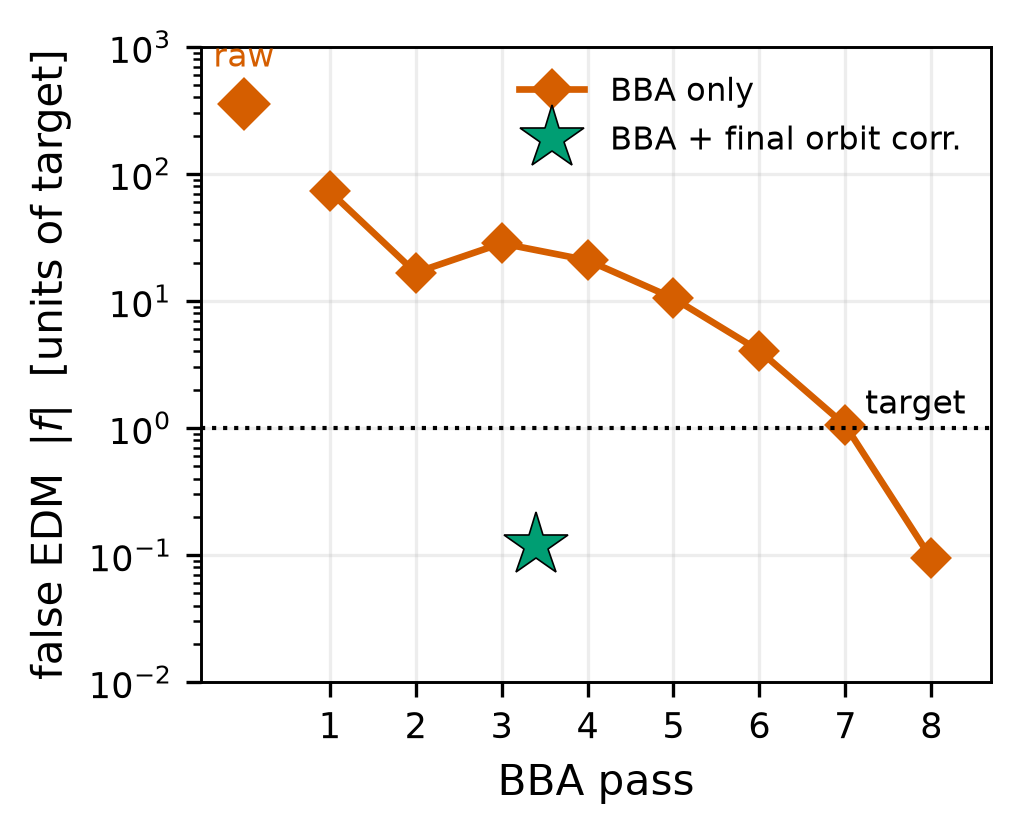
\includegraphics[width=\columnwidth]{fig_orbit_bba_convergence.png}
\caption{Demet-tabanlı hizalama sahte EDM'i platosuz biçimde hedefin altına
sürükler (ölçülen-matris BBA, muhafazakâr $\%1$ rms gradyan hatası,
$\approx\!\%5$ $\beta$-vuruşu, sekiz geçiş, C++ izleme). Baklava: sahte EDM $|f|$,
ham makineden ($356\times$ hedef) sekiz BBA geçişi boyunca; üçüncü geçişten sonra
tekdüze düşer ve sekizincide hedef-altına ($0{,}09\times$) geçer. Plato yapmaz;
iniş yalnızca yavaştır, çünkü BBA simetrik artığı mıknatıs mıknatıs öğütür ve
tek-demet tepki-matrisi inversiyonunun ulaşamadığı yörünge-kör bileşene ulaşır. Son
bir yörünge düzeltmesi yörünge-görünür antisimetrik artığı kolektif olarak kaldırır
ve sekiz yerine yaklaşık üç geçişte hedefe ulaşır (yeşil yıldız: beş-tohum topluluğu,
medyan $0{,}07\times$, hepsi hedef-altı).}
\label{fig:bbaconv}
\end{figure}

Hizalama rotası içindeki ortaya çıkan tablo tutarlı ve tamamlayıcıdır:
\emph{tek-demet yörünge düzeltmesi Denk.~(\ref{eq:channels})'in antisimetrik
kanallarını kaldırır ama simetrik tabanı bırakır (karşı-dönen artık $47\times$'te
oturur); sıfır-arayan BBA, tek-demet yörünge düzeltmesinin göremediği simetrik
kanala ulaşır ve yeterince yinelendiğinde hedefe tek başına ulaşır; ikisini
birleştirmek birkaç geçişte ulaşır.} Simetrik kanalın aslında tümüyle yörünge
düzeltmesinin erişiminin ötesinde olmadığı --- iki karşı-dönen demeti birlikte
düzeltmenin BBA'sız ona ulaştığı --- Böl.~\ref{sec:orbitreach}'in konusudur.
İşbölümü bir \emph{hassasiyet} meselesidir de: her mıknatıs-başına sıfır geçişi
$\sim\!\mu$m seviyesinde bir ölçüm tabanı taşır (artık nefes ve yönlendirme-modeli
hatası), dolayısıyla BBA'yı tek başına yinelemek o tabana ancak yavaş yaklaşır;
antisimetrik artık ise mıknatıs-başına hiçbir ölçüm gerektirmez --- yörünge onu
doğrudan ve rezonant biçimde yükseltilmiş gösterir ve onu bir kesik-SVD düzeltmesiyle
(yukarıdaki ``derinlik'' tekil-değer kesimidir) kolektif sıfırlamak, mıknatıs
mıknatıs ölçmekten çok daha hassastır. Tablo~\ref{tab:chain} zinciri özetler. Uç
nokta beş kaçıklık tohumu üzerinde nitelenir: sabit bir kesik-SVD derinliğinde
($\mathrm{rcond}=0{,}01$, bir kez seçilir ve tohum başına ayarlanmaz) beşi de
hedefin altına iner, medyan $0{,}07\times$ ve en kötü $0{,}22\times$
(Şek.~\ref{fig:suppression}). Sahte EDM tohumdan tohuma saçılan işaretli, bilineer
bir nicelik olduğundan (Şek.~\ref{fig:channels}), sağlam ifade herhangi tek bir sayı
değil, tüm topluluğun hedefin altına bastırılmasıdır. Herhangi bir demet-tabanlı
hizalamada olduğu gibi, her kampanyanın tekrarlanabilirliği --- merkezleri bulmak
için kullanılan gradyan modülasyonu altında manyetik merkezlerin kararlılığı ---
yordamın ne sıklıkla yinelenmesi gerektiğini belirleyen bir donanım girdisidir;
onu nicelendirmek bu izleme çalışmasının kapsamı dışındadır. Deney için öngörülen
hava-çekirdekli (demirsiz) kuadrupoller, manyetik histerezisten muaf olduklarından
bu açıdan elverişlidir.

\begin{table}[tb]
\caption{$\sigma = 10~\mu$m'de bastırma zinciri (tek demet, izleme). Satır 2 ve 4
beş-tohum topluluklarıdır: satır 2, yörünge düzeltmesinden sonra karşı-dönen demet
farkının medyanı (yayılım $0{,}6$--$72\times$) ve son satır tam şemanın dağılımı
(sabit $\mathrm{rcond}=0{,}01$, tüm tohumlar hedef-altı, medyan $0{,}07\times$); ham
ve BBA satırları temsili deseni izler (ham $356\times$). Eşdeğer EDM
$1~\text{nrad/s} \leftrightarrow 10^{-29}\,e\!\cdot\!$cm kullanır.}
\label{tab:chain}
\small
\begin{ruledtabular}
\begin{tabular}{lcc}
Aşama & $|f|$ / hedef & EDM [$e\!\cdot\!$cm] \\
\hline
ham                            & $356\times$ & $\sim4\times10^{-27}$ \\
tek-demet yörünge düz.\ $+$ CW/CCW & $\sim47\times$ & $\sim5\times10^{-28}$ \\
BBA (ölçülen yönlendirme)      & $17$--$28\times$ & $\sim2\times10^{-28}$ \\
BBA $+$ son yörünge düz.       & $0{,}03$--$0{,}22\times$ & $\lesssim10^{-29}$ \\
\end{tabular}
\end{ruledtabular}
\end{table}

\subsection{Polarite dört-katlısı ve bedeli}
\label{sec:fourfold}

Ref.~\cite{omarov} simetrik kanala herhangi bir yörünge okumasından geçmeyen bir
rotayla ulaşır: \emph{bütün odaklayıcı kuadrupollerin polaritesini ters çevirmek}
ve karşı-dönen farkı yinelemek [Denk.~(C2)]. Demet yönü ve manyetik gradyanın
eşzamanlı tersine çevrilmesi altında Lorentz kuvveti $q\,\bm v\times\bm B$
değişmez, dolayısıyla ters kafeste karşı-dönen bir demet, nominal kafeste
birlikte-dönen bir demetin yörüngesini yeniden izler; manyetik-kafes sahte EDM'i iki
konfigürasyon arasında özdeştir ve dört-katlı kombinasyonda iptal olur, elektrik-alan
EDM'i ise iptal olmaz. Bunu doğrudan doğruluyoruz: dört-katlı kombinasyon \emph{hem}
simetrik hem antisimetrik desenin sahte EDM'ini kestirici tabanına
($0{,}009\times$ ve $-0{,}017\times$ hedef) kaldırır; aynı $\bm v\times\bm B$
simetrisine uyan kuadrupol dönüklüğünden ya da $\beta$-vuruşundan bağımsız olarak.

Dört-katlı iptal ilkede tamdır ve BBA'nın tek başına hedefin üstünde bıraktığı
simetrik kanala ulaşır --- ama bedelsiz değildir. İki polarite durumu aynı anda
depolanamaz; sırayla ölçülürler ve iptal, makinenin her ikisinde \emph{aynı}
kaçıklığı sunmasını gerektirir. Sahte EDM bilineer olduğundan
[Denk.~(\ref{eq:bilinear})], durumlar arasındaki herhangi bir değişimin bıraktığı
artık, çevredeki kaçıklık ile değişimin \emph{çarpımıyla} orantılıdır, dolayısıyla
aynı drift daha iyi-hizalı bir makinede daha az bedel getirir: BBA'dan sonra
(simetrik rms $\sim\!2~\mu$m) $1~\mu$m'lik simetrik konfigürasyonlar-arası bir drift
$0{,}07\times$ hedef bırakır, oysa ham $10~\mu$m'lik makinede hedefin onlarca katını
üretir. Daha genel olarak, ters gradyanları yeniden üretmede $\varepsilon$ kesirli
bir hata, büyük ortak-mod sinyalinin bir kesrini EDM kanalına kaçırır; $10~\mu$m'lik
bir makinede $\varepsilon=10^{-3}$ gradyan asimetrisi yaklaşık $1\times$ hedef
bırakır. Önemli olan drift simetrik olandır, yörüngeye görünmezdir, dolayısıyla
dört-katlı, tersine-çevirme boyunca \emph{kararlı tutulan} BBA-seviyesinde bir
simetrik hizalama talep eder. Bu --- hizalama kampanyaları, ardışık ikinci
konfigürasyon ve aralarındaki kararlılık gereksinimi --- sonraki bölümün yalnız-yörünge
yönteminin kaldırdığı işletme bedelidir.

% ═══════════════════════════════════════════════════════════════════

\section{Simetrik bileşene karşı-dönen yörünge düzeltmesiyle ulaşmak}
\label{sec:orbitreach}

\subsection{Standart düzeltmeden sonraki artık}
\label{sec:chain}

Her iki düzlemde $\sigma = 10~\mu$m'lik rasgele kaçıklıklar için ham sahte EDM,
hedefin $10^{3}$ katı mertebesindedir [Denk.~(\ref{eq:target})]; bu makale boyunca
kullanılan temsili bir desen $356\times$ verir. Standart yörünge düzeltmesi ---
kapalı yörüngeyi yönlendirme düzelticileriyle düzleştirmek --- topluluk medyanını
yaklaşık sekiz kat azaltır; Böl.~\ref{sec:polarity}'de tartışılan karşı-dönen demet
farkıyla birleştirildiğinde artık, hedefin yaklaşık $47\times$'idir
($\approx 5\times10^{-28}\,e\!\cdot\!$cm), $\sigma^{2}$ olarak ölçeklenir
(Şek.~\ref{fig:suppression}). Yörünge düzeltmesi böylece etkilidir ama yeterli
değildir; artık Böl.~\ref{sec:mechanism}'in simetrik tabanıdır ve bu bölümün geri
kalanı tek-demet bir düzeltmenin ona neden ulaşamadığını ve iki karşı-dönen demeti
birlikte düzeltmenin nasıl ulaştığını gösterir.

\begin{figure}[tb]
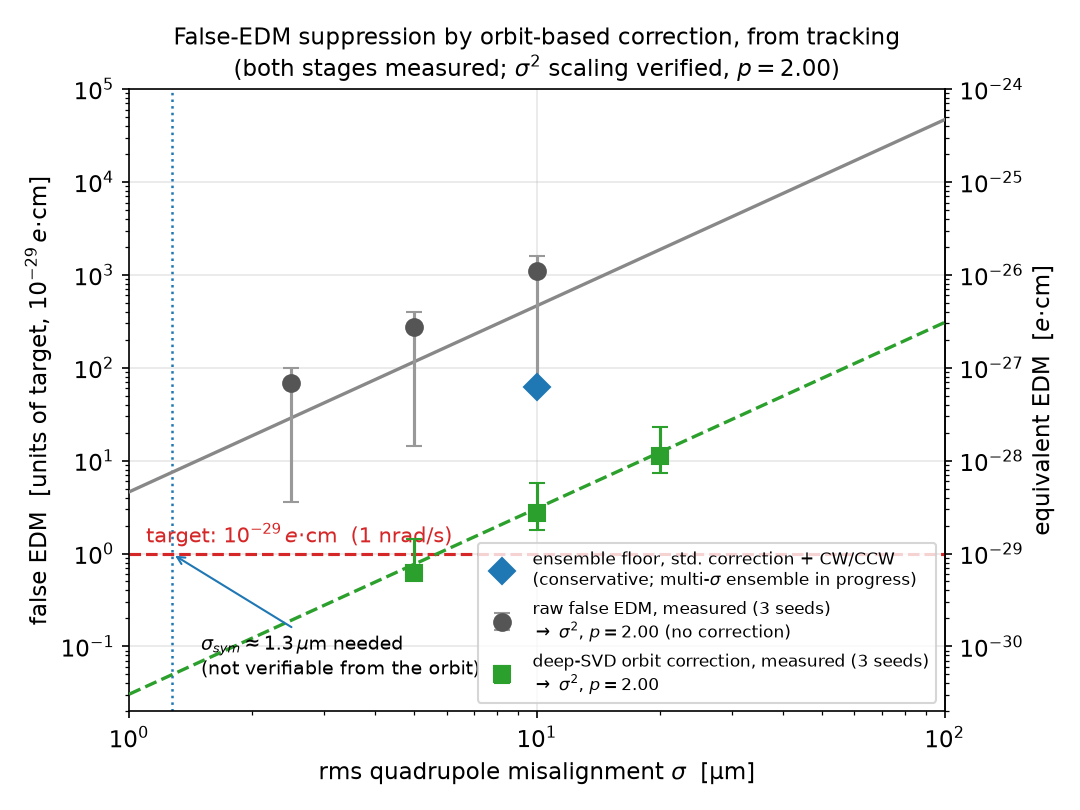
\includegraphics[width=\columnwidth]{fig_orbit_suppression.png}
\caption{Tek-demet sahte EDM'in rms kaçıklığa karşı değişimi (izleme; medyan ve tam
yayılım). Daireler: ham desen (düzeltme yok). Kareler: yalnız yörünge düzeltmesi;
antisimetrik kanalları kaldırır ama simetrik tabanı bırakır --- $\sigma=10~\mu$m'de
hâlâ hedefin birkaç katı. İkisi de $\sigma^2$ olarak ölçeklenir (her aşamada
$p=2{,}00$), geometrik-faz kökenini doğrulayarak; uydurma bir mutlak tabanı değil
ölçeklemeyi doğrular, çünkü sabit $\sigma$'da sahte EDM desenin
simetrik/antisimetrik içeriğine göre bir büyüklük mertebesinden fazla değişir
(Böl.~\ref{sec:bilinear}). Simetrik tabana $\sigma=10~\mu$m'de iki bağımsız rotayla
hedefin altında ulaşılır (sabit $\mathrm{rcond}=0{,}01$). Yıldız: demet-tabanlı
hizalama ardından bir yörünge düzeltmesi (medyan $0{,}07\times$, en kötü
$0{,}22\times$, beş tohum; Tablo~\ref{tab:chain}). Baklava: kalibre bir referansa
karşı iki-demet karşı-dönen yörünge düzeltmesi, BBA yok, gerçekçi $\%1$
$\beta$-vuruşunda (medyan $0{,}043\times$, en kötü $0{,}62\times$, on beş tohum;
Tablo~\ref{tab:twobeam} ve Böl.~\ref{sec:polarity}). Baklava, tek artık
$\tfrac12|f_{\rm CW}-f_{\rm CCW}|$'dir; iki rota da artığı hedefin belirgin biçimde
altına yerleştirir.}
\label{fig:suppression}
\end{figure}

\subsection{Klasik yörünge yöntemlerinin ulaşamama nedenleri: iki engel}
\label{sec:obstructions}

Başaran ölçümü sunmadan önce, başarısız olanları ve nedenlerini özetliyoruz.
Hepsi, kaçıklıkları (kritik olarak simetrik parçalarını da) yörünge okumalarından
geri çatmaya çalışır. Gerçekçi hata modeli statik BPM ofsetleri ($\sim\!100~\mu$m
her biri, bir monitörün gerçek eksene göre elektronik sıfırı), beyaz BPM gürültüsü
($\sim\!1~\mu$m okuma başına, ortalamayla azaltılabilir) ve tutarlı bir optik-model
hatası içerir ($\beta$-vuruşu, izleyicide kuadrupol başına kesirli gradyan hataları
olarak uygulanır; aşağıdaki testlerde kullanılan $\%1$ rms işletme noktası bu
kafeste $\approx\!\%5$ rms $\beta$-vuruşu üretir (tepe $\approx\!\%10$), tedirgeli
tek-tur Twiss'ten hesaplanır, öyle ki LOCO-düzeltilmiş optiğin tipik $\sim\!\%1$--$2$
değerine göre eğer bir şeyse kötümserdir).

\emph{Engel 1 --- koşullanma (fark-yörünge inversiyonu).} Bütün kuadrupol
gradyanlarını iki ayar arasında modüle edip yörüngeleri çıkarmak, statik BPM
ofsetlerini tam olarak iptal eder ve doğrusal bir sistem $\Delta y = \Delta R\,\Delta q$
bırakır. Hatasız durumda inversiyon tamdır. Zayıflığı koşullanmadır:
$\mathrm{cond}(\Delta R) = 3{,}7\times10^{4}$, zayıf yönler tam olarak simetrik olanlardır
($\Delta R$'ye uygulanan Şek.~\ref{fig:modes}'deki aynı simetrik-kesir analiziyle
kurulmuş), dolayısıyla geri-çatma hataları ilgilenilen bileşen boyunca yükseltilir.
İnversiyonu düzenlileştirmek --- kesik SVD ya da Tikhonov sönümü --- burada yardım
etmez: kesme tam olarak simetrik yönleri atar, gürültü yükseltmelerini aranan
bileşenin tam bir sapmasıyla takas eder. Bu, herhangi bir optik hatası
\emph{olmadan} bile doğrudur: yalnız lock-in gürültü tabanında koşullanma, simetrik
geri-çatma hatasını antisimetriğin yaklaşık on katına yükseltir (Ek~\ref{app:inversion}).
Beyaz gürültü senkron algılamayla yenilebilir --- $\sim\!1$~kHz'de modüle edip
ortalamak dakikalar içinde $\sim\!14$~nm etkin gürültüye ulaşır --- ama tutarlı bir
optik-model hatası yenilemez: o her ortalamada özdeştir ve daha en yumuşak gerçekçi
$\beta$-vuruşunda bile --- $\%1$ ($\%0{,}2$ rms gradyan hatası), bir LOCO
düzeltmesinin başardığı en iyisi --- geri-çatılan simetrik bileşen gerçeğin birkaç
katıdır ($41$-$\mu$m'lik bir sinyale karşı standart testimizde $\sim\!110~\mu$m),
antisimetrik bileşen ise doğru kalır (Ek~\ref{app:inversion}); hata $\beta$-vuruşuyla
büyür ve Böl.~\ref{sec:bba}--\ref{sec:polarity}'nin yapıcı testleri için benimsenen
$\%5$ işletme noktasında ($\%1$ rms gradyan hatası) daha da büyüktür, öyle ki
simetrik kanal tüm gerçekçi aralık boyunca kaybedilir. Sınır tutarlı olduğundan BPM
teknolojisinden bağımsızdır; SQUID-tabanlılar dahil düşük-gürültülü alıcılar
integrasyon süresini kısaltır ama tabanı oynatmaz. Aynı yapısal nokta bir sınır
olarak da ifade edilebilir: statik ofsetleri iki-ayar farkıyla iptal eden her
kestirici, iptalin bedelini bir $\|\Delta R^{-1}\| \sim \|R^{-1}\|/\varepsilon_g$
yükseltmesiyle öder; burada $\varepsilon_g$ göreli ayar farkıdır.

\emph{Engel 2 --- optik nefes (genlik olarak okunan modülasyon).} Her kuadrupole
kendi modülasyon frekansını atayıp BPM'lerde frekans-başına genliği okumak ---
Ref.~\cite{marti}'nin ac-BBA kavramı --- doğrudan, inversiyonsuz bir okuma vaat
eder: merkezi demetten $o_i$ kadar ofsetli bir kuadrupol, gradyanı modüle edildiğinde
$o_i$ ile orantılı dipol-benzeri bir saptırma (feed-down tekmesi) izler. Yöntem bu
halkada öğretici bir nedenle başarısız olur (Ek~\ref{app:breathing}). Sorun,
modüle edilen kuadrupolün kendisinin küresel etkisidir. Bir kuadrupol odaklayıcı bir
elemandır: gradyanını $\%2$ bile değiştirmek \emph{tüm} halkanın tune'unu ve odak
fonksiyonlarını hafifçe kaydırır. Diğer tüm kuadrupollerin ofsetlerince inşa edilen
ve $\sim\!0{,}37$~mm rms'te aranan $\sim\!0{,}9$-$\mu$m'lik feed-down sinyalinin
birkaç yüz katı olan mevcut kapalı yörünge, bu hafifçe değişmiş odaklamadan yeniden
taşınır ve her BPM'de birkaç $\mu$m oynar. Bu küresel tepki --- Böl.~\ref{sec:bbareal}'de
zaten karşılaşılan optik \emph{nefes} --- tam olarak ölçülen kuadrupolün modülasyon
frekansında görünür, dolayısıyla hiçbir frekans filtresi onu sinyalden ayıramaz. O
zaman bir BPM'de demodüle edilen okuma kuadrupolün kendi feed-down'u değildir:
en-kötü-kuplajlı kuadrupol için mevcut yörüngenin nefesinin sürüklediği genlik,
kendi ofsetinin üreteceğinin $266$ katıdır, dolayısıyla ofset için tersine
alınacak sayı \emph{diğer} mıknatısların yörüngesince domine edilir ve bu
tek-frekans okumada hiçbir sabit kalibrasyon ondan doğru niceliği geri kazanmaz
(Ek~\ref{app:breathing}). Nefes modülasyonla tutarlı olduğundan ortalanıp gitmez ve
idealize bir modelde onu kaldırmak kusursuz geri-çatmayı geri getirir, ki bu,
başarısızlığı tümüyle bu mekanizmaya bağlar.

Bu iki engelin ortak sonucu yapısaldır. İnversiyon ve genlik-okuma ailelerindeki
her teknik için sınırlayıcı etki tutarlıdır --- $\beta$-vuruşuyla yükseltilen
koşullanma ya da optik nefes --- ve tutarlı etkiler ortalanıp azalmaz.
\emph{Simüle edilen model içinde, SQUID-tabanlı BPM'ler dahil hiçbir BPM teknolojisi
bu tabanları değiştirmez.} Bu ifadenin kapsamını vurguluyoruz. O, ele alınan
kestirici sınıflarının yapısal bir özelliğidir; sınıf-seviyesi argümanlarla
(koşullanma sınırı ve nefes teriminin tutarlılığı) sistematik simülasyonla birlikte
kurulmuştur; her düşünülebilir yörünge-tabanlı ölçüm için bir bilgi-teorik
imkânsızlık iddiası değildir. Gerçekten de, sonraki bölümün karşı-dönen düzeltmesi,
simetrik bileşene ulaşan, bu sınıfların dışında yörünge-tabanlı bir ölçümdür.

\subsection{Karşı-dönen toplam körlüğü kırar}
\label{sec:polarity}

Ref.~\cite{omarov}'un gerçek EDM'i ayıran ölçümü karşı-dönen farktır: EDM
demet-tersine-çevirme altında tektir, dolayısıyla
$(dS_y/dt)_{\rm CW}-(dS_y/dt)_{\rm CCW}$'de hayatta kalır, ortak-mod sistematikler
iptal olur [Denk.~(C1)] ve aynı anda depolanan iki demet farkı drift-serbest kılar.
Saf demet-tersine-çevirme-çift bir sahte EDM burada yok olurdu; geometrik faz
olmaz, çünkü iki demet hafifçe farklı kapalı yörüngeler sürer ve bir
demet-tersine-çevirme-\emph{tek} artık hayatta kalır. $\sigma=10~\mu$m'de beş tohum
üzerinde bu artık, saf simetrik bir kaçıklık için hedefin $4$--$60\times$'i (medyan
$22\times$) ve saf antisimetrik biri için $38$--$496\times$'i (medyan $175\times$)'dır;
\emph{tek} bir demetin yörüngesini düzeltmek antisimetrik parçayı kaldırır ama farkı
$\sim\!45\times$'te bırakır (medyan, $0{,}1$--$67\times$; Tablo~\ref{tab:twobeam}).

Tek düzeltmenin neden yetmediği ve onun ötesine geçmenin yolu, ikisi de iki yörünge
tepki matrisi arasındaki ilişkide içerilir. Onlar neredeyse zıttır: yatay bir
kuadrupol yer değiştirmesi için yazınca, $R_{\rm CW}=-R_{\rm CCW}+\Delta$,
işaret-çevrilmiş parça domine eder ve bir yön-ortak artık $\Delta$ hayatta kalır.
İşaret çevrimi başat etkidir, çünkü kaçık bir kuadrupol sabit bir dipol gibi davranır
(feed-down alanı yer değiştirmeyle belirlenir, demetle değil) ve Lorentz kuvveti
$q\,\bm v\times\bm B$ karşı-dönen demetin hızıyla ters döner, dolayısıyla aynı tekme
iki demeti zıt yönde saptırır. Ters çevirmediği şey mıknatıslar arası betatron faz
ilerlemesidir; bu, belirli bir QF/QD/deflektör sırasına sahip bir halkada her eleman
etrafında ayna-simetrik değildir; o karşılıksızlık artık $\Delta$'dır. Frobenius
normunda yatay düzlem için $\lVert\tfrac12(R_{\rm CW}-R_{\rm CCW})\rVert=33{,}8$ ve
$\lVert\tfrac12(R_{\rm CW}+R_{\rm CCW})\rVert=7{,}3$, bir $\%21$'lik $\Delta$; dikey
düzlem aynıdır ($45{,}8$ ve $9{,}7$, $\%21$), dolayısıyla etki yatay bükümün bir
ürünü değildir. Bu neredeyse-zıtlık tam olarak, iki yörüngenin \emph{ayrımının} ---
referans denetim zincirinin izlediği gözlenebilir (Böl.~\ref{sec:obstructions}) ---
simetrik bileşene neden kör olduğudur: fark $R_{\rm CW}-R_{\rm CCW}\approx-2R_{\rm CCW}$
antisimetrik-görünür parçayı ikiye katlar ve simetrik görünürlüğü, birim-normlu
simetrik ile antisimetrik desenlerin tepkisinin Frobenius-norm oranı
$\lVert R\,P_{\rm sym}\rVert/\lVert R\,P_{\rm anti}\rVert$, $0{,}19$'dur --- tek bir
demetten ($0{,}24$) daha iyi değil. \emph{Toplam} ise, başat antisimetrik tepkiyi
iptal eder ve simetrik bileşeni açığa serer: simetrik görünürlüğü $1{,}01$ ve
koşullanma sayısı $30$'dur. Tek demetin ve ayrımın ikisinin de yoksun olduğu bilgi,
iki karşı-dönen yörüngenin toplamında taşınır.

Şekil~\ref{fig:cwccwsum} bunu gerçek-uzayda gösterir. Temsili antisimetrik bir
kaçıklık için iki demet, büyük genlikleri toplamda iptal olan neredeyse-ayna-görüntüsü
kapalı yörüngeler sürer (sıfır azimutal kaymada korelasyon $-0{,}95$), küçük bir
artık bırakarak. Simetrik bir kaçıklık için iki yörünge ise birkaç BPM kaymış
\emph{aynı} şekildir --- korelasyonları sıfır kaymada sıfıra yakındır ama
$\sim\!5$-BPM'lik bir kaymada $+0{,}94$'e çıkar, artık $\Delta$'yı oluşturan
yön-ters betatron faz ilerlemesinin bir sonucu --- dolayısıyla toplam iptal olmaz
ve orijinal simetrik yörüngenin ölçeğinde hayatta kalır. Toplam böylece tam olarak
tek bir demette simetriği maskeleyen antisimetrik yörüngeyi bastırır ve tek bir
demetin göremediği simetrik yörüngeyi korur.

\begin{figure*}[tb]
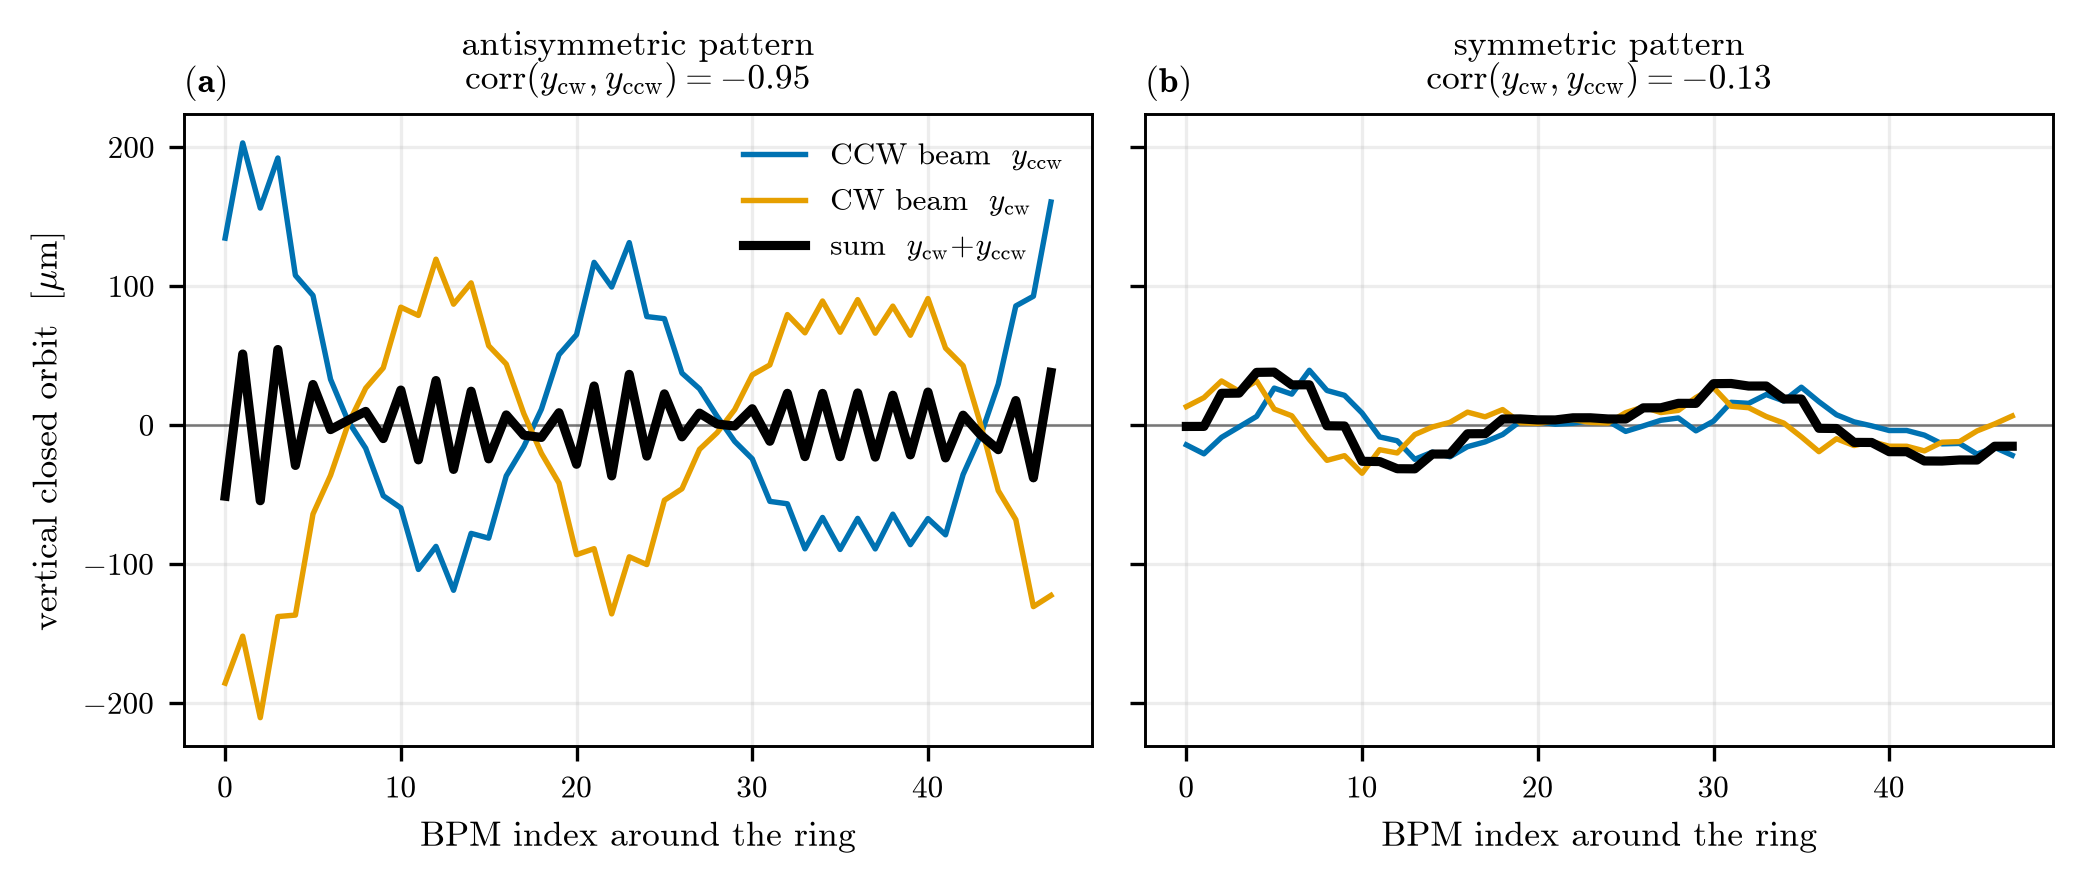
\includegraphics[width=\textwidth]{fig_orbit_cwccw.png}
\caption{İki karşı-dönen demetin aynı $10~\mu$m-rms kaçıklık için dikey kapalı
yörüngeleri (analitik tepki matrisleri). (a) Antisimetrik bir desen büyük,
neredeyse-zıt yörüngeler ($\mathrm{corr}=-0{,}95$) sürükler, bunlar toplamda
(siyah) iptal olur. (b) Simetrik bir desen küçük yörüngeler sürükler; bunlar birkaç
BPM kaymış aynı şekildir (sıfır kaymada $\mathrm{corr}\approx0$); toplamları iptal
olmaz ve tek tek yörüngelerin ölçeğinde kalır. Toplam böylece tek bir demeti
boğan antisimetrik yörüngeyi kaldırır ve tek bir demetin çözemediği simetrik
yörüngeyi tutar.}
\label{fig:cwccwsum}
\end{figure*}

\subsection{İki yörüngeyi birlikte düzeltmek ve performans}
\label{sec:joint}

İki yörüngeyi birlikte düzeltmek bunu kullanır. Donmuş-spin halkasında saat-yönünde
ve saat-yönü-tersi demetler aynı anda depolanır ve birbirinin içinden karşı-dönerek
geçer; çok sayıda bunch ile demet-konum monitörleri iki türü ayrı zaman
pencerelerinde çözer, dolayısıyla iki kapalı yörüngenin BPM-başına toplamı doğrudan
elde edilir. İki tepki matrisini yığmak, $S=[R_{\rm CCW};\,R_{\rm CW}]$, ve her iki
yörüngeyi düzleştiren tek en-küçük-kareler düzeltmesini çözmek, onların toplam ve
farkını birlikte kullanmakla eşdeğerdir; dolayısıyla simetrik bileşene toplam
üzerinden erişimi vardır. Etki bir koşullanma etkisidir, düzenlileştirmeyle
keskinleşir. Tek-demet yatay matris (izlemeden) $\mathrm{cond}(R_{\rm CCW})=135$
($228$ dikey) değerine sahiptir; sözde-tersin kesmesinde ($\mathrm{rcond}=10^{-2}$)
en zayıf on yedi tekil yön eşiğin altına düşer ve atılır, her biri simetrik-baskındır
--- onları tutmak simetrik düzeltmedeki BPM gürültüsünü $\sim\!7\times$ yükseltirdi,
Böl.~\ref{sec:obstructions}'ün inversiyon no-go'suyla aynı engel. Yığılmış matris
$\mathrm{cond}(S)=73$ ($118$ dikey) değerine sahiptir: hiçbir yön eşiğin altına
düşmez ve simetrik modlar $0{,}7\times$'lik bir gürültü yükseltmesiyle düzeltilir.
İkinci demet no-go'yu aşmaz; simetrik bileşeni, hiçbir tek demetin taşımadığı toplam
bilgisini sağlayarak, no-go'nun bahsettiği gürültü tabanının üstüne kaldırır.

Düzeltmeyi neyin gerçekleştirdiği önemlidir ve aynı fizikçe belirlenir. Çözülen
nicelik bir \emph{manyetik-merkez kayması} kümesidir $c$ --- hizalanabilir kuadrupol
başına bir, düzlem başına 47 --- Böl.~\ref{sec:bbaproc}'nün BBA'sında olduğu gibi,
dipol yönlendirmesiyle değil, kuadrupol bobinleri arasındaki bir akım asimetrisiyle
gerçekleştirilir. Ayrım esastır. Bir merkez kayması, kaçıklığın kendisinin geometrik
bir değişimidir, $m\to m-c$, iki demet için \emph{aynı}, dolayısıyla simetrik bileşeni
kaynağında sıfırlayabilir; bir dipol yönlendirme düzelticisi ise kuadrupol yerine
demeti kaydırır ve Lorentz tekmesi demet hızıyla ters döndüğünden onun demet--merkez
ofseti üzerindeki etkisi yön-tektir --- bir demetin yörüngesini düzleştirebilir ama
iki demeti aynı anda kuadrupollere ortalayamaz. İki-demet düzeltmesi bu nedenle
hizalama programının zaten gerektirdiği donanım olan merkez-kayması aktüatörlerini
varsayar; yeni bir düzeltici sınıfı değil, yalnızca iki yörüngenin yeni bir
kullanımını getirir.

Sahte EDM için sonuç kesindir. Ham $10~\mu$m'lik makinede, demet-tabanlı hizalama
olmadan ve yörünge kalibre bir referansa karşı ölçülerek, iki-demet yörünge
düzeltmesi simetrik kaçıklık artığını $\sim\!5{,}5~\mu$m'den (tek demet)
$0{,}1$--$0{,}7~\mu$m'e --- BBA'nın ulaştığı $\sim\!2~\mu$m'de ya da altında
(Böl.~\ref{sec:bba}) --- indirir ve her iki karşı-dönen sahte EDM'i birlikte tabana
sürükler, öyle ki tek fark hedefin altına iner.\footnote{Şema iki karşı-dönen
yörüngeyi paylaşılan BPM'lerde okur, referans tasarımın ayrımlarını izlemek için zaten
yaptığı gibi, bunch zamanlamasıyla ayırt edilerek; o ayrımdan farklı olarak iki
mutlak yörüngeyi kullanır, farklarını değil. $14$~nm rakamı dakikalar boyunca senkron
ortalamayla ulaşılan etkin nokta-başına gürültüdür (Böl.~\ref{sec:obstructions}) ve
yalnızca düzeltmenin beyaz-gürültü tabanı olarak girer.} Tablo~\ref{tab:twobeam}
tutarlı optik hatasına bağımlılığı verir. Tüm gerçekçi aralık boyunca düzeltme
sağlam biçimde hedef-altıdır: tipik LOCO işletme noktasında ($\%1$ $\beta$-vuruşu,
$\%0{,}2$ rms gradyan hatası) tek artık on beş tohum üzerinde medyan hedefin
$0{,}043\times$'idir, hepsi hedef-altı (en kötü $0{,}62\times$) ve iyi-düzeltilmiş
bir makinede ($\%0{,}5$ $\beta$-vuruşu) medyan $0{,}03\times$'tir. Yalnızca LOCO'nun
sunduğunun üstünde, gerçekçi olmayan büyük bir $\%5$ $\beta$-vuruşunda tutarlı artık
önem kazanmaya başlar (medyan $0{,}66\times$, beşin üçü hedef-altı) ---
Böl.~\ref{sec:obstructions}'ün fark-yörünge inversiyonunu yenen aynı
tutarlı-model-hatası tabanı, ama burada iki-demet düzeltmesi bir inversiyon değil
iyi-koşullu bir ileri düzleştirme olduğundan yumuşamış. $\%1$-$\beta$-vuruşlu
makineye $0{,}2$~mrad modellenmemiş bir kuadrupol dönüklüğü eklemek sonucu değiştirmez
(medyan $0{,}12\times$): dönüklük, $\bm v\times\bm B$ simetrisi altında bile bir
manyetik-kafes etkisidir, dolayısıyla iki demete eşit katkı yapar ve tek farkta iptal
olur.\footnote{Buradaki dönüklük sahte-EDM ölçümüne, başat geometrik-faz kanalına
girer; iki enine yörüngenin ikinci-derece kuplajı (kuplajsız) düzeltmeye
beslenmez, dolayısıyla test $\bm v\times\bm B$ argümanının tanımladığı başat kanalı
sınırlar.}

\subsection{Sınır: BPM-ofset dejenerasyonu}
\label{sec:limit}

Bu rakamlar kalibre bir referans varsayar ve bu kayıt bir teknik ayrıntı değildir.
Gerçek BPM'lerin statik elektriksel ofsetleri --- $\sim\!100~\mu$m, referans denetim
zincirinin farklama ile kaldırdığı aynı ofsetler (Böl.~\ref{sec:obstructions}) ---
bu şemayı keskin ve öğretici bir nedenle bozar. Ofset $b$ iki demete ortaktır,
dolayısıyla farklarında iptal olur ama toplamlarına \emph{iki katı} eklenir --- ve
toplam tam olarak simetrik bileşeni taşıyan kanaldır. Simetrik kaçıklık ile statik
ofset bu nedenle karşı-dönen toplamda \emph{dejeneredir}: birini açığa çıkaran
izdüşümün tam da diğerini açığa çıkarır ve hiçbir tek-anlı yörünge ölçümü onları
ayırmaz. İzlemede $100~\mu$m'lik kalibre edilmemiş ofsetleri geri koymak tek artığı
$0{,}043\times$'ten $\sim\!200\times$ hedefe döndürür (Tablo~\ref{tab:twobeam}) ve
tolerans şiddetlidir --- simetrik artık ofset rms'inin $0{,}96\times$'i olarak büyür,
dolayısıyla hedef-altı işletme, ofsetlerin yalnızca BBA'nın sağladığı
kuadrupol-merkez seviyesinde, $\lesssim\!0{,}5~\mu$m'e bilinmesini gerektirirdi.
İki-demet düzeltmesi böylece mutlak konum referansı ihtiyacını kaldırmaz; o ihtiyacı
tek, temiz biçimde ifade edilmiş bir dejenerasyonda yoğunlaştırır. Bu sınırın nasıl
aşıldığı --- drift diferansiyel olduğundan --- Böl.~\ref{sec:operation}'in konusudur.

\begin{table}[tb]
\caption{Ham $\sigma=10~\mu$m'lik makinede karşı-dönen yörünge düzeltmesi (BBA yok;
$14$~nm BPM gürültüsü; izleme). Tek artık, hedef biriminde karşı-dönen fark
$C=\tfrac12|f_{\rm CW}-f_{\rm CCW}|$'dir. Üst blok: kalibre bir referansa karşı
düzeltme, tutarlı optik hatasına karşı --- iki-demet düzeltmesi gerçekçi aralık
boyunca hedef-altıdır ve yalnızca gerçekçi olmayan büyük bir $\%5$ $\beta$-vuruşunda
bozulur. Alt: $100~\mu$m'lik kalibre edilmemiş statik BPM ofsetleriyle tek artık
$\sim\!200\times$'e döner, çünkü ofset ve simetrik kaçıklık karşı-dönen toplamda
dejeneredir --- düzeltme, statik ofsetin özdeş iptal olduğu \emph{diferansiyel}
(drift) yörünge üzerinde etki etmedikçe. LOCO işletme noktası 15 tohum üzerindedir,
diğer noktalar 5.}
\label{tab:twobeam}
\small
\begin{ruledtabular}
\begin{tabular}{lcc}
$\beta$-vuruşu ($\sigma_g$), referans & tek-demet & iki-demet (medyan) \\
\hline
$\%0{,}5$ ($\%0{,}1$), kalibre        & $\sim\!46\times$ & $0{,}03\times$ \;(5/5) \\
$\%1$ ($\%0{,}2$, LOCO), kalibre     & $\sim\!32\times$ & $0{,}043\times$ \;(15/15) \\
$\%1$ $+\,0{,}2$~mrad dönüklük, kalibre & $\sim\!45\times$ & $0{,}12\times$ \;(5/5) \\
$\%5$ ($\%1$), kalibre             & $\sim\!29\times$ & $0{,}66\times$ \;(3/5) \\
\hline
$\%1$, $100~\mu$m ofset (mutlak)   & $\sim\!650\times$ & $198\times$ \;(0/5) \\
$\%1$, $100~\mu$m ofset (diferansiyel) & --- & $0{,}043\times$ \;(15/15) \\
\end{tabular}
\end{ruledtabular}
\end{table}

% ═══════════════════════════════════════════════════════════════════

\section{Şemanın işletimi: drift ve zaman bütçesi}
\label{sec:operation}

Bir hizalama sonucu ancak makinede hayatta kalırsa faydalıdır. Kuadrupol konumları
--- ısıl olarak ve zemin hareketiyle~\cite{rossbach} --- sürekli drift eder,
düzeltilmiş duruma sürekli rasgele kaçıklık yeniden yükleyerek. Bunu, rms $\sigma_{\rm d}$
taze rasgele ofsetler ekleyip sahte EDM'i yeniden ölçerek simüle ettik.

İşletme tablosunu yöneten ayrım iki kaçıklık bileşeni arasındadır. Tek-demet yörünge
geri beslemesi driftin yalnızca antisimetrik parçasını kaldırır, dolayısıyla onunla
tek başına sahte EDM $\sigma_{\rm d}$ için $\sim\!5~\mu$m'e kadar hedef-altı kalır
($2~\mu$m'de $0{,}05\times$, $5~\mu$m'de $0{,}3$--$0{,}6\times$), ama yavaşça biriken
\emph{simetrik} parça ona görünmezdir ve referans programda demet-tabanlı hizalamanın
tekrarlanmasını zorlar. Karşı-dönen düzeltmenin hakkını verdiği yer burasıdır.
Böl.~\ref{sec:orbitreach}'te gösterildiği gibi, iki-demet düzeltmesi simetrik
bileşene ulaşır --- ve drift için kritik olarak, bunu diferansiyel yörünge üzerinde
herhangi mutlak kalibrasyon olmadan yapar: drift $\Delta q = q(t)-q(t_0)$'dır, karşılık
gelen yörünge değişimi $\Delta y = R\,\Delta q$ statik BPM ofsetinden serbesttir (o,
iki zaman arasında iptal olur) ve karşı-dönen toplamı $\Delta q$'nun simetrik
parçasını açığa çıkarır. Ofset özdeş biçimde iptal olduğundan, diferansiyel düzeltme
vektörü ofset-serbest olanla \emph{aynıdır} --- dolayısıyla izlenen performans ayrı
bir yaklaşıklık değil, tam olarak Tablo~\ref{tab:twobeam}'in ofset-serbest
topluluğudur --- ve her çevrim yeniden-referanslar, öyle ki iptal bir koşu boyunca
hata biriktirmez. $\Delta y$ üzerinde sürekli bir iki-demet geri beslemesi böylece
\emph{simetrik} drifti, yalnızca antisimetriği değil, o ofset-serbest seviyede tutar.
Başlangıç mutlak hizalaması yine bir kampanya gerektirir --- BBA ya da polarite
dört-katlısı --- simetrik bileşeni Böl.~\ref{sec:orbitreach}'in ofset dejenerasyonuna
karşı ayarlamak için; ama onun \emph{sürdürülmesi}, simetrik driftin aksi hâlde talep
edeceği tekrarlanan yeniden-hizalama, sürekli geri beslemeyle değiştirilir.

Zaman bütçesi izler. Başlangıç hizalaması tek-seferlik bir bedeldir --- bir yörünge
düzeltmesiyle kapatılan birkaç-geçişli bir BBA kampanyası yarım gün mertebesindedir
($47~\text{mıknatıs}\times2~\text{düzlem}\times2~\text{demet konumu}\times
2~\text{gradyan ayarı}\approx400$ yörünge alımı geçiş başına, her biri
$\sim\!10$~s) --- sonrasında iki-demet geri beslemesi veri alımı sırasında ek maliyetsiz
çalışır ve simetrik drift için başka kampanya planlanmaz. O zaman deneyin başat zaman
ölçeği istatistiksel olan kalır: polarimetri nrad/s seviyesine ancak aylardan bir yıla
uzanan koşuyla ulaşır~\cite{polarimeter} ve sürekli düzeltme ona hiçbir şey eklemez.
BPM ofsetinin statik olduğu varsayımı üzerine bir söz. Diferansiyel, iki ardışık
okumaya ortak ofseti iptal eder, dolayısıyla yalnızca aralarındaki ofset
\emph{değişimi} hayatta kalır ve o değişim --- yavaş bir ısıl ya da elektronik drift
--- simetrik kanala küçük bir kaçıklık gibi sızar. Sürekli (yuvarlanan) işletimde bu
çevrim-başına kaçaklar bir rasgele yürüyüş olarak birikir: $N$ çevrimden sonra simetrik
artık $\approx 0{,}96\,\dot b\,\tau_c \sqrt{N}$'dir; burada $\dot b$ ofset drift hızı,
$\tau_c$ çevrim süresidir (katsayı $0{,}96$ yukarıdaki aynı ofset-den-simetriğe
izdüşümdür ve $\sqrt{N}$ ölçeklemesini izleyicide doğruluyoruz). Sayısal olarak,
dakikada bir düzeltilen $1~\mu$m/gün'lük bir ofset drifti bir günde yalnızca
$\sim\!0{,}03~\mu$m ve sürekli bir yıllık koşuda $\sim\!0{,}5~\mu$m ---
tutarlı-optik tabanı --- sızdırır; herhangi büyüklükte \emph{statik} bir ofset tam
olarak iptal olur. Gereksinim böylece ofsetin küçük olması değil, düzeltme
kadansına kıyasla yavaş drift etmesidir; gerçekçi BPM'ler bunu büyüklük mertebeleriyle
karşılar. Burada modellenmeyen iki donanım girdisi nicelendirilmeyi bekler: başlangıç
BBA'sının gradyan modülasyonu altında manyetik-merkez kararlılığı (tekrarlanabilirliği)
ve diferansiyel tepkiye bir $\beta$-vuruşu gibi giren monitör-başına bir BPM kazanç
hatası ($\%1$ kazanç $\sim\!0{,}6~\mu$m simetrik artık bırakır, dolayısıyla yüzde
seviyesinde kazanç kalibrasyonu yeterlidir).

% ═══════════════════════════════════════════════════════════════════

\section{Sonuçlar}
\label{sec:conclusions}

Simetrik-hibrit proton EDM halkası için önerilen denetim programı, demet-tabanlı
hizalamayı bir dört-katlı ölçümle --- her iki kuadrupol polaritesinde karşı-dönen
fark --- eşleştirir; bu, kuadrupol-kaçıklık sahte EDM'ini iptal eder~\cite{omarov}.
Semplektik spin izleme kullanarak, tek başına yörünge düzeltmesinin bu görevi ne
kadar taşıyabileceğini sorduk ve yanıt, sahte EDM'in bilineer dört-kanallı yapısıyla
ve iki kaçıklık bileşeninin keskin biçimde farklı yörünge görünürlüğüyle belirlenir.

(1) Sahte EDM iki enine kaçıklık deseninin bilineer bir fonksiyonelidir
[Denk.~(\ref{eq:channels})], izlemede $\%0{,}1$ seviyesinde doğrulanmış ve
yörünge-görünür bir antisimetrik parçaya ile yörünge tepkisinin mod mod iki
büyüklük mertebesine kadar daha zayıf olduğu bir simetrik parçaya ayrılır. Bu
nedenle bir rms toleransıyla nitelenmez: sabit $\sigma$'da desene göre bir büyüklük
mertebesinden fazla değişir ve bir düzeltme yordamı büyüklüğü değil, artığın yattığı
\emph{bileşeni} değiştirir.

(2) Referans çözüm hedefe ama bir işletme bedeliyle ulaşır. Sıfır-arayan BBA,
yörünge inversiyonunun ulaşamadığı simetrik bileşene ulaşır --- her manyetik
merkezi global bir tersle değil, yerel bir sıfır geçişiyle konumlandırır --- ve
yeterince yinelendiğinde sahte EDM'i tek başına hedefin altına sürükler (tekdüze,
sekizinci geçişe kadar $0{,}09\times$; plato yoktur), ama yavaşça; tek bir son
yörünge düzeltmesi yörünge-görünür antisimetrik artığı kolektif olarak kaldırır ve
onun yerine yaklaşık üç geçişte hedefe ulaşır. BBA, elektrik deflektörlerinin yatay
odaklamasını ihmal eden idealize bir kafesin sağlamadığı sadık bir \emph{yatay}
yönlendirme modeli gerektirir. Polarite dört-katlısı tabana bir adımda ulaşır, ama
yalnızca makine ardışık iki polarite durumunda aynı simetrik hizalamayı sunarsa;
yörüngeye görünmez $1~\mu$m'lik bir simetrik konfigürasyonlar-arası drift, sahte
EDM'i hedefin onlarca katına yeniden açar.

(3) Karşı-dönen yörünge düzeltmesi simetrik bileşene yörüngeden ulaşır, tek bir
dejenerasyona tabi. Tek-demet bir ölçüm ulaşamaz: simetrik kaçıklık ona neredeyse
görünmezdir ve referans zincirin izlediği karşı-dönen \emph{ayrım} daha iyi değildir,
iki neredeyse-zıt yörüngenin \emph{farkı} olduğundan. \emph{Toplamları} ise simetrik
bileşeni tümüyle açığa çıkarır (ayrım için $0{,}2$'ye karşı simetrik görünürlük
$1{,}0$) ve iki yörüngeyi kalibre bir referansa karşı birlikte düzeltmek bunu
kullanır: ham $10~\mu$m'lik makinede karşı-dönen fark, gerçekçi $\%1$ $\beta$-vuruşunda
on beş tohum üzerinde medyan hedefin $0{,}043\times$'ine iner, hepsi hedef-altı,
$\beta$-vuruşuyla ve $0{,}2$~mrad modellenmemiş kuadrupol dönüklüğüyle değişmez. Ne
var ki aynı toplam statik BPM ofsetini simetrik kaçıklıkla orada dejenere biçimde
taşır ($100~\mu$m kalibre edilmemiş ofsetler artığı $\sim\!200\times$'e döndürür);
dolayısıyla iki-demet düzeltmesi, bir BBA kampanyasının ya da dört-katlının hâlâ
kurması gereken mutlak referans ihtiyacını kaldırmaz.

(4) Kaldırdığı şey \emph{periyodik} yeniden-hizalamadır ve işletme rolü budur. Drift
diferansiyeldir: statik ofset yörünge \emph{değişimi} $\Delta y = R\,\Delta q$'de
iptal olur; onun karşı-dönen toplamı driftin simetrik parçasını ofset bulaşması
olmadan açığa çıkarır, dolayısıyla sürekli bir iki-demet geri beslemesi simetrik
hizalamayı --- tek-demet geri beslemesinin göremediği ve referans programda BBA'nın
tekrarlanmasını zorlayan bileşeni --- ofset-serbest seviyede süresiz tutar. Başlangıç
hizalaması tek-seferlik bir bedeldir; sürdürülmesi ise sürekli ve bedelsizdir ve zaman
bütçesi polarimetrinin istatistiksel ölçeğince domine edilir~\cite{polarimeter}.
Nicelendirilecek kalan öğeler tutarlı-optik tabanı (yönteme karşı $\sim\!\%1$
$\beta$-vuruşuna kadar sağlam) ve diferansiyel tepkiye bir $\beta$-vuruşu gibi giren
monitör-başına bir BPM kazanç hatasıdır --- $\%1$ kazanç $\sim\!0{,}6~\mu$m simetrik
artık ekler, optik tabanıyla kıyaslanabilir, dolayısıyla standart yüzde seviyesinde
kalibre edilen BPM kazançları yeter.

Bütün sayılar, sekstupolsüz doğrusal bir modelde, proton EDM deneyi için tasarlanan
simetrik-hibrit halkaya~\cite{omarov} atıfta bulunur. Niteliksel ile niceliksel
arasındaki bir ayrım akılda tutulmalıdır. Yapısal sonuçlar --- görünürlük ayrımı,
bilineer kanal ayrışımı ve simetrik bileşenin karşı-dönen farkta değil toplamda
açığa çıkması --- güçlü-odaklamalı halkalarda ortak olan değişken-gradyanlı odaklamaya
dayanır ve bu tür başka kafeslere taşınmasını bekliyoruz. Onları nicelendiren sayısal
değerler --- simetrik görünürlükler (fark için $0{,}19$, toplam için $1{,}01$),
koşullanma sayıları (tek-demet $135$, yığılmış $73$), yön-ortak artık ($\%21$) ve
bastırma çarpanları --- bu kafesin özellikleridir ve başka bir kafes için yeniden
hesaplanırdı; genel olduğunu iddia ettiğimiz bu sayılar değil, yapıdır. Başlıca açık
öğeler, herhangi bir BBA çapraz-kontrolünün gradyan modülasyonu altındaki
manyetik-merkez kararlılığı (burada modellenmeyen donanım tabanı) ve diğer kafes
varyantlarında doğrulamadır.

İzleme ve analiz kodu, tepki matrisleri ve figürler ile tabloların arkasındaki
veriler makul talep üzerine yazarlardan edinilebilir.

% ═══════════════════════════════════════════════════════════════════

\begin{acknowledgments}
%
\end{acknowledgments}

% ═══════════════════════════════════════════════════════════════════
\appendix

\section{Fark-yörünge inversiyonu ve lock-in okuması}
\label{app:inversion}

Böl.~\ref{sec:obstructions}'ün birinci engelinin (koşullanma) niceliği burada
kaydedilir. Fark-yörünge inversiyonu statik ofsetleri iptal eder ama $\Delta R$'nin
$3{,}7\times10^{4}$'lük koşullanmasını miras alır. Şekil~\ref{fig:lockin}, senkron
algılama gürültü tabanında (10~nm) simetrik ve antisimetrik bileşenlerin geri-çatma
hatasını $\beta$-vuruşuna karşı gösterir: daha $\%1$'de simetrik hata sinyali aşar
ve sıfır $\beta$-vuruşunda bile koşullanma simetrik hatayı antisimetriğin bir
büyüklük mertebesi üstünde bırakır. Kesik-SVD ya da Tikhonov düzenlileştirmesi
yardım etmez, çünkü kesme tam da simetrik yönleri atar.

\begin{figure}[tb]
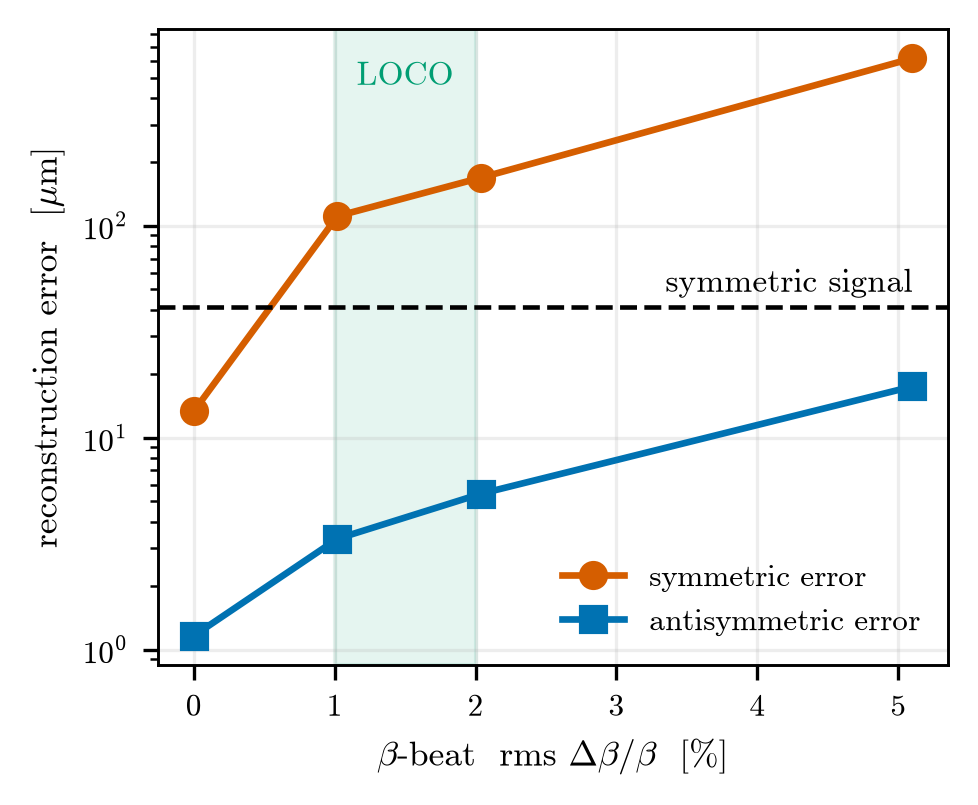
\includegraphics[width=\columnwidth]{fig_orbit_lockin.png}
\caption{Senkron-algılama gürültü tabanında (10~nm, 40 tohum) fark-yörünge
inversiyonu: simetrik ve antisimetrik bileşenlerin geri-çatma hatası $\beta$-vuruşuna
karşı (sürükleyen gradyan hatası $\sigma_g$ $\approx\!5\times$ daha küçüktür). Kesikli
çizgi simetrik sinyalin kendi büyüklüğünü, gölgeli bant gerçekçi LOCO aralığını
($\sim\!\%1$--$2$ $\beta$-vuruşu) işaretler. Daha $\%1$'de simetrik hata sinyali
aşar; sıfır $\beta$-vuruşunda bile koşullanma simetrik hatayı antisimetriğin bir
büyüklük mertebesi üstünde bırakır, girdi ile geri-çatma arasındaki Pearson
korelasyonu yanıltıcı biçimde yüksek kalsa da.}
\label{fig:lockin}
\end{figure}

\section{Kuadrupol-başına genlik modülasyonu ve optik nefes}
\label{app:breathing}

Böl.~\ref{sec:obstructions}'ün ikinci engelinin (optik nefes) niceliği burada
kaydedilir. Şekil~\ref{fig:breathing}, kuadrupol-başına gradyan modülasyonunun
genlik olarak okunmasında geri-çatılan ofsetleri gerçek ofsetlere karşı gösterir:
optik nefes yapay olarak kaldırıldığında geri-çatma tamdır, ama nefes mevcutken
onunla ilişkisizdir --- modülasyonla tutarlı olan nefes ortalanıp azalmaz.

\begin{figure}[tb]
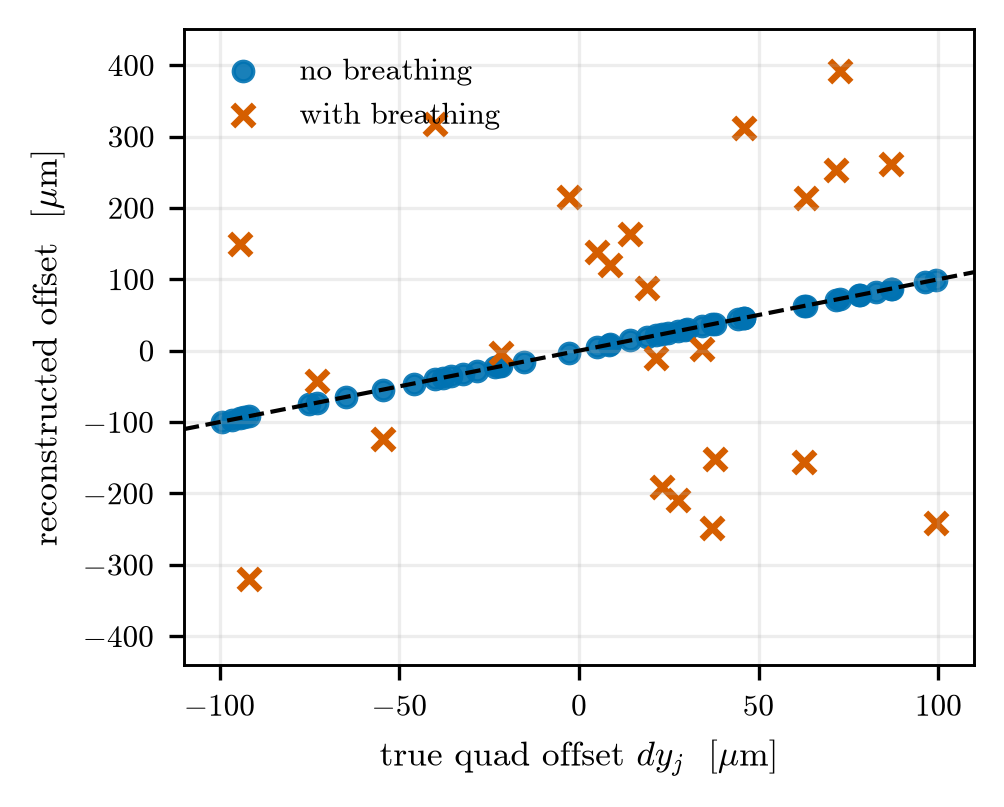
\includegraphics[width=\columnwidth]{fig_orbit_breathing.png}
\caption{Kuadrupol-başına gradyan modülasyonunun genlik olarak okunması: geri-çatılan
ofsetlere karşı gerçek ofsetler. Optik nefes yapay olarak kaldırıldığında geri-çatma
tamdır, ama nefes mevcutken onunla ilişkisizdir --- modülasyonla tutarlı olan nefes
ortalanıp azalmaz.}
\label{fig:breathing}
\end{figure}

\section{Tune'u yükseltmek ve SQUID BPM'ler}
\label{app:tune}

Simetrik kick harmoniğine doğru betatron tune'unu yükseltmek, o bileşeni ilkece
görünür kılardı, ama durgun bantla sınırlanır ($Q \leq 12$, yavaş değişen simetrik
modların gerektirdiği $Q \geq 16$'ya karşı) ve her hâlükârda sahte EDM'in kendisini
dik biçimde yükseltir (ölçülen $\sim\!g^{3}$). Ayrıca Böl.~\ref{sec:obstructions}'ün
tabanları tutarlıdır, dolayısıyla BPM teknolojisinden bağımsızdır: SQUID-tabanlılar
dahil düşük-gürültülü alıcılar integrasyon süresini kısaltır ama tabanı oynatmaz.

% ═══════════════════════════════════════════════════════════════════
\begin{thebibliography}{99}

\bibitem{omarov}
Z.~Omarov, H.~Davoudiasl, S.~Hac{\i}\"omero\u{g}lu, V.~Lebedev,
W.~M.~Morse, Y.~K.~Semertzidis, A.~J.~Silenko, E.~J.~Stephenson, and
R.~Suleiman,
``Comprehensive symmetric-hybrid ring design for a proton EDM experiment at
below $10^{-29}\,e\!\cdot\!$cm,''
Phys.\ Rev.\ D \textbf{105}, 032001 (2022).

\bibitem{haciomeroglu2017}
S.~Hac{\i}\"omero\u{g}lu and Y.~K.~Semertzidis,
``Systematic errors related to quadrupole misplacement in an all-electric
storage ring for proton EDM experiment,''
arXiv:1709.01208.

\bibitem{chung1993}
Y.~Chung, G.~Decker, and K.~Evans,
``Closed orbit correction using singular value decomposition of the response
matrix,''
in \emph{Proceedings of PAC 1993}, p.~2263.

\bibitem{wegscheider}
S.~Wegscheider, J.~Vilsmeier, \emph{et al.},
``Inverse modeling of circular lattices via orbit response in the presence
of degeneracy,''
Phys.\ Rev.\ Accel.\ Beams \textbf{26}, 032803 (2023).

\bibitem{marti}
Z.~Mart\'{\i}, G.~Benedetti, U.~Iriso, and A.~Franchi,
``Fast beam-based alignment using ac excitations,''
Phys.\ Rev.\ Accel.\ Beams \textbf{23}, 012802 (2020).

\bibitem{huang}
X.~Huang,
``Simultaneous beam based alignment measurement for multiple magnets,''
arXiv:2203.14869.

\bibitem{mirza}
S.~H.~Mirza, R.~Singh, P.~Forck, and H.~Klingbeil,
``Closed orbit correction at synchrotrons for symmetric and near-symmetric
lattices,''
Phys.\ Rev.\ Accel.\ Beams \textbf{22}, 072804 (2019).

\bibitem{ziemann}
V.~Ziemann and M.~Ziemann,
``Noninvasively improving the orbit response matrix while continuously
correcting the orbit,''
arXiv:2104.05300.

\bibitem{rossbach}
J.~Rossbach,
``Closed-orbit distortions of periodic FODO lattices due to plane ground
waves,''
Part.\ Accel.\ \textbf{23}, 121 (1989).

\bibitem{polarimeter}
F.~M\"uller \emph{et al.} (JEDI Collaboration),
``A new beam polarimeter at COSY to search for electric dipole moments of
charged particles,''
arXiv:2010.13536.

\end{thebibliography}

\end{document}
